\title{Campaign Contributions and Bureaucratic Oversight: A Case Study of the Federal Energy Regulatory Commission}

\author{Eleanor Neff Powell\thanks{Booth Fowler Associate Professor, University of Wisconsin-Madison} \and Devin Judge-Lord\thanks{Postdoctoral Fellow, Harvard University}\and Justin Grimmer\thanks{Professor, Stanford University}}

\date{\today}

\documentclass{article}
\usepackage[margin=1in]{geometry}

% === bibliography package ===
\usepackage{natbib}

% === to do notes===
% \usepackage[colorinlistoftodos, prependcaption]{todonotes} % to use \todo 

% === fonts, captions, and spacing===
%\usepackage{csquotes}
\usepackage{rotating}
\usepackage{setspace}
%\usepackage{filecontents}
\usepackage[labelformat=empty]{caption}
%\usepackage[title]{appendix}
\usepackage{subcaption}
\usepackage{lmodern, amssymb,amsmath, graphicx, hyperref}
\hypersetup{
    colorlinks=true,
    linkcolor=blue,
    filecolor=magenta,      
    urlcolor=cyan,
    citecolor = black
}
\urlstyle{same}  % don't use monospace font for urls
    
% === figures===
\graphicspath{{Figs/}}

\begin{document}

\maketitle
% \tableofcontents

% \bigskip
% \href{https://judgelord.github.io/correspondence/gh-pages/FERCsummary.html}{Project Summary} | 
% \href{https://docs.google.com/document/d/1fJxjXjAyRL9vX-16fSsH29anXZc-W74GMf_7BSgWkws/edit}{Codebook} |
% \bigskip

\texttt{This paper was prepared for the Association for Environmental Studies and Sciences Conference.  \href{https://github.com/judgelord/correspondence/raw/master/FERC/FERCpaper2019.pdf}{The most recent draft is available here.} \bigskip \bigskip \bigskip}


\begin{abstract}
\noindent 

We use letters legislators that write to the Federal Energy Regulatory Commission to study congressional attempts to influence bureaucratic decisions. Analizing thousands of letters from legislators to the agency sent over nearly two decades, we find that these letters are filled with specific references to companies that legislators seek to assist or about which the legislator's constituents have complaints.  We explore which legislators seek to influence the agency, on whose behalf they make requests, and what outcomes they attempt to influence.  Finally, we match these letters with campaign finance records to see whether legislators' behavior correlates with the campaign contributions they receive from the energy industry.  We find that Republicans and those who receive money from the energy-sector write relatively more letters on behalf of energy companies, but not on behalf of constituents, while Democrats write comparatively more letters in opposition to energy companies. %To some extent, these results capture a general focus on energy issues, but there is some evidence that elected officials who receive more money from the industry in a cycle write advocate more on behalf of companies in the following legislative session. 

\end{abstract}


\newpage
\doublespacing
\section{Introduction}

Concern over the potential for campaign contributions to influence elected officials has been a central question in American politics for several decades.  Much of the academic research in this area has focused on whether campaign contributions influence legislators' roll call votes.  These numerous studies have produced somewhat mixed results. On the whole, however, the answer appears to be no: that, most of the time, campaign contributions don't influence how a member votes in the context of a roll call vote.  The focus on roll call votes is unsurprising given the availability of the data, but the availability and visibility of roll call votes also make them a poor vehicle for those seeking to quietly influence the government decisions without drawing scrutiny from journalists, activists, or constituents. 

Compared to the intense scrutiny of roll call votes, scholars have paid much less attention to congressional advocacy and oversight activities, such as when legislators write letters or emails to government bureaucrats urging them toward or against some decision.\footnote{This has begun to change in the last few years with recent studies by  \citet{MillsKalafHuges2015, Ritchie2017, Lowande2018JOP, LowandeRitchieLauterbach2018, JudgeLordGrimmerPowell2018}.} While these letters are technically subject to federal open records laws, the disclosure process is often slow and difficult, meaning that, in practice, these letters rarely see the light of day and are highly unlikely to draw public scrutiny. Thus, securing a letter from an individual legislator may be a preferred vehicle for those seeking to quietly influence specific government decisions through campaign contributions.  

In this paper, we deeply examine legislators' letters written to one agency -- the Federal Energy Regulatory Commission (FERC).  We explore whether these letters to the commission appear motivated by constituency service or campaign contributions. Specifically, we investigate whether campaign contributions from political action committees of corporations in the energy sector are correlated with legislator's letter-writing to the commission on behalf of those companies. We find that Republicans and those who receive money from energy-sector write relatively more letters on behalf of energy companies, but not on behalf of constituents, while Democrats write comparatively more often in opposition to energy companies. To some extent, these results capture a general focus on energy issues; writing all kinds of letters, not just pro-business letters, is positively correlated with energy-sector campaign contributions both in particular electoral cycles and legislative sessions and over a legislator's career. Yet, there is some evidence that elected officials who receive more money from the industry in a cycle write more on behalf of companies than against them in the following legislative session. % TODO, directly test this hypothesis with "ratio of pro-business letters" as the DV

\section{Studying the Influence of Campaign Contributions on Congressional-Bureaucratic Relations}

Attempting to study the influence of campaign contributions on political outcomes is fraught with methodological and observational challenges.  As two of us (Powell and Grimmer) have written previously, two of the primary challenges to studying the influence of money on the most visible form of congressional behavior (roll call votes) are legality and visibility \citep{PowellGrimmer2016}. Regarding legality, as the \citet{USOGE2013} describes, if something of value is given, offered, or promised with the intent ``to influence any official act,'' it is illegal behavior on the part of the contributor. Similarly, on the recipient side, if a public official demands, seeks, receives, or accepts an item of value, it is illegal behavior on the part of the legislator.  Given threats of prosecution and jail time, we might expect both contributors and politicians to avoid public actions that could be construed in such a way.  

And even if an action is legal, it might still create the appearance of impropriety and therefore create an incentive for legislators to obscure it.  To the extent that both campaign contributors who might be seeking favors and elected officials who seek campaign contributions are concerned about appearances, we might expect elected officials to avoid taking visible public actions that could be viewed as corrupt.  Rather, both the elected officials and contributors should prefer actions that achieve the same end but through less observable means. As we elaborate in the following section, much of the research on money in politics has focused on highly visible outcomes such as roll call votes---the least likely places that these actors would want to connect themselves.  In contrast, congressional letter-writing to bureaucratic agencies is much less visible and thus a better place to look for the influence of money in politics.  These letters, which we have obtained through laborious Freedom of Information Act requests and web scraping, are not easily accessible to the public, and both legislators and campaign contributors may reasonably assume that these documents will never be subject to public scrutiny.  Certainly, they are rarely accessed, and thus those actors hoping to fly under the radar may prefer them to more overt legislative acts. 

Furthermore, many government decisions that affect businesses are made by agencies rather than Congress. If legislators aim to help a donor, their oversight powers may thus often be more useful then their legislating powers. As an independent commission with broad discretion over policy, permitting, and enforcement ranging from price controls on electricity markets to the construction interstate natural gas pipelines, FERC decisions major consequences to the energy sector.

Finally, before reviewing previous research on the influence of money in American politics, we must add a necessary note of caution about the conclusions we can draw in this paper.  This project is an observational study that looks at the correlation between campaign contributions and attempts to influence the Federal Energy Regulatory Commission through legislative letters.  We are limited by our data and can only use cross-sectional designs.  That said, our results suggest interesting patterns that deserve to be interrogated with data that enables more robust research designs. %Given our research design, we cannot draw conclusive causal findings but rather can explore relationships that might be promising areas for future research with a more robust causal design.  

\subsection{The Uneven Evidence for the Influence of Money in American Politics}

Extensive scholarship examines the influence of money on American politics. And yet, there is only mixed evidence that money influences the legislative process. The literature has demonstrated that donors appear to contribute in ways consistent with short term access seeking \citep{Snyder1992, RomerSnyder1994, PowellGrimmer2016, Barber2016, FouirnaiesHall2018}.  

Yet, the evidence that legislators undertake actions explicitly for donors is limited.  There are some exceptions. First, there is a literature on contributions to congressional committees, where it is clear that corporations donate to pivotal legislators' congressional committees \citep{PowellGrimmer2016, BerryFowler2016}. 
In addition to showing that donors appear interested in short-term access-seeking and contribute to those members influential in policy areas relevant to their business interests, work by \citet{KallaBroockman2016} shows that donors are more likely to get meetings with key members of Congress.  This finding is again consistent with this short-term access-seeking behavior. Yet there is a considerable gap between taking a meeting with a donor and actually advancing their interests. Overall, this literature fails to connect contributions to specific actions by legislators. 

Scholars have also investigated whether campaign contributions influence roll-call votes in Congress \citep{AnsolabehereFigueiredoSnyder2003, RoscoeJenkins2005, CalcagnoJackson1998, Chappell1982, ConleyMcCabe2012, EngelJackson1998, Fleisher1993, Grenzke1989, MilyoPrimoGroseclose2000, JonesKeiser1987, KauRubin1982, LanLot1990,Lessig2011, MoorePowellReeves2013, Neustadtl1990, Saltzman1987, Stratmann1991, Stratmann1992, Stratmann1995, Stratmann2002, Wawro2001, Wright1985, Wright1989, Wright1990, Wright2004}.  Although the findings aren't entirely consistent in this area, the vast majority of studies fail to find an impact of campaign contributions on roll call voting. Given that both campaign contributors and elected officials may be concerned by issues of legality and visibility, highly visible roll call votes are an unlikely place to find a correlation between campaign funding and legislator behavior. 

There is relatively little work specifically examining the links between campaign contributions, legislators, and the bureaucracy.\footnote{One notable exception is \citet{GordonHafer2005}, which develops a formal model of the strategic and signaling complexity of these relationships and finds that large corporate donors overseen by the Nuclear Regulatory Commission are both less compliant and less monitored by the bureaucracy.} 
This is surprising because it is an intuitive location to look for campaign donors seeking influence; these less visible areas of policymaking are where we would expect to find corporate influence \citep{Hall1996}.  Further, bureaucrats have a strong incentive to reply to legislators' requests.  They have this incentive because legislators have both oversight powers over federal agencies and because legislators can influence agencies' budgets.  And as a result, we expect that donors may contribute to legislators to subsidize their efforts creating a relationship between campaign donations and behavior. 

% \subsection{How Corporations Can Make Campaign Contributions}

% Let us now turn from the existing literature on the influence of money to the question of how corporations can make campaign contributions.  The campaign financing landscape has undergone a substantial transformation over the last several decades. Perhaps the area of greatest change is the regulation surrounding how corporations (and other business entities) can engage in political activity.  As the Federal Election Commission's \textit{Campaign Guide for Corporations and Labor Unions} describes: 

% \singlespacing
% \begin{quotation}
% ``The Federal Election Campaign Act (the Act) generally prohibits corporations ... from using their general treasury funds to make contributions to federal candidates, federal accounts of political party committees, and other political committees (PACS). 52 U.S.C. \S 30118(a). They may, however, fund independent expenditures, contribute to political committees established solely to finance independent expenditures (e.g., Super PACs), contribute to the non-contribution accounts of Hybrid PACs, and establish separate segregated funds (SSFs),''\citep[][pg.1]{FEC2018}.
% \end{quotation}
% \doublespacing

% Thus, there are a variety of methods that companies can engage in political activities.  In this paper, we will focus on what the Federal Election Commission calls Separate Segregated Funds (SSFs), which are more commonly called corporate-sponsored political action committees (PACs) \citep{FEC2018}.  These corporate PACs may raise money in order to make contributions to federal candidates as well as and expenditures on behalf of federal candidates and committees.  The full name of the company (also called the connected organization or sponsoring company or organization) must appear in the name of the company's PAC. The connected organization is the organization (corporation) that establishes, administers, or financially supports the PAC.  The Connected Organization may exercise control over the corporate PAC.  Note that if a connected organization has parent companies/subsidiaries, those names don't need to be included in the name of the SSF. 

% %SSFs set up by parent/subsidiary corporations are automatically considered affiliates and bound by a single set of contribution limits.  SSF affiliates must be listed on its Statement of Organization.

\section{Theory: Why Legislators May Act on Behalf of Donors at FERC}

While the literature on constituency service has primarily focused on legislators assisting their constituents, in this section, we explain why legislators are likely to also act on behalf of corporate interests, particularly at FERC.  In line with Arnold's (1979) argument of the anticipated benefits of particularistic spending, elected officials have two kinds of incentives.  Elected officials have incentives to advance the interests of potential donors. Projects authorized by FERC may have direct financial benefits to a legislator's district, providing an opportunity to claim credit \citep{Arnold1979, GriWesMes14}. Likewise, projects are opportunities for businesses to profit, and thus an opportunity for elected officials to demonstrate their value to potential corporate funders. Within the set of potential energy projects, it is reasonable to expect that elected officials will advocate those in their district and those of potential donors.

%Arnold's insights about the anticipated consequences of actions also suggest the converse dynamic: elected officials ought to be less likely to advocate against projects sponsored by potential donors and more likely to advocate against projects when they anticipate opposition from constituents in their district. 


% \subsection{Why Might Legislators Act on Behalf of Constituents?}

% One of the earliest and most comprehensive academic descriptions of constituency service comes from Richard Fenno in his classic book \emph{Home Style: House Members in Their Districts}. As Fenno describes:

% \begin{displayquote}
% Many activities can be incorporated under the rubric of `district service,' or `constituent service,' but the core activity is providing help to individuals, groups, and localities in coping with the federal government.  Individuals need someone to intercede with the bureaucracies handling their veterans' benefits, social security checks, military status, civil service pension, immigration proceedings, and the like.  Private groups and local governments need assistance in pursuing federal funds for water and sewer projects, highways, dams, buildings, planning, research and development, small business loans, and so forth \citep[pg. 101]{Fenno1978}.
% \end{displayquote}

% While the definition that Fenno presents is broad, the central element is clear: assisting constituents (individuals or groups) in interacting with government agencies.  Fenno's description is consistent with how \citet[pg. 2]{CainFerejohnFiorina1987} characterize constituency service as acting as an ``ombudsman'' for constituents vis-a-vis the administrative state.  These scholarly definitions of constituent service from \citep{Fenno1978} and \citet{CainFerejohnFiorina1987} are consistent with how legislators understand the concept today, and according to a recent Congressional Research Service Report constituency service ``is commonly considered a representational responsibility'' \citep{Eckman2017}.  Before proceeding to discuss why legislators perform constituency service in the following section, it is worth noting that this definition of constituency service is an expansive one that encompasses both individual casework activity (e.g. requests for assistance with a social security check) and district- or group-level advocacy. It does not hinge on a precise definition of which individuals and groups count as constituents. Representatives may advocate for groups that are organized and intense demanders of government benefits or protections (e.g. support for a local union facing a factory closing) or merely linked by a common fate (e.g. general support for hurricane recovery aid in the district). The key distinction in this notion of constituent service is that it is an act of service to a particular individual or group at a particular time, rather than a broad or enduring policy that may apply to many groups over time. 

% To understand why legislators engage in constituency service, we turn to the broader literature on what motivates Members of Congress?  The classic answer comes from \citet{Mayhew1974}. In \emph{Congress: The Electoral Connection}, Mayhew argues that re-election is the primary (or at least the proximate) motivation because it is a necessary step to achieve other goals (such as policy or power within Washington). Constituency service activity has traditionally been viewed as a way to improve one's re-election prospects by assisting individual (or groups of) constituents.  As \citet*{CainFerejohnFiorina1984} and \citet*{CainFerejohnFiorina1987} describe, constituency service helps to build a member's ``personal vote'' which they defined to be the ``portion of a candidate's electoral support which originates in his or her personal qualities, qualifications, activities, and record,'' \citep*[][pg. 9]{CainFerejohnFiorina1987}. In their survey of congressional staffers, \citet{CainFerejohnFiorina1987} found that the overwhelming majority of staffers believed that constituency service activity has electoral payoffs by positively contributing to a legislator's ``personal vote.'' 

\subsection{Why Might Legislators Act on Behalf of Donors?}

To answer why legislators might act on behalf of donors, we return again to \citet{Mayhew1974}'s argument that re-election is the proximate motivation of most legislators because it is necessary to achieve other goals.  While constituency service -- helping individual voters-- may incrementally (voter by voter) improve a legislator's electoral prospects, the campaign contributions a legislator receives can be used in a myriad of ways to potentially boost a legislator's campaign.  While the political science literature disagrees on the impact of campaign spending and political campaigns more generally on electoral outcomes, few politicians would dispute the widely held view among political practitioners that campaign funds help members win re-election.  

\section{Why Study the Federal Energy Regulatory Commission?}
Like many agencies within the federal bureaucracy, The Federal Energy Regulatory Commission (FERC) makes policy and enforcement decisions that have major consequences for jobs, lives, profits, and the cost of the commodities it regulations. FERC regulates electricity markets, oil and gas pipelines, hydropower projects, and liquified natural gas export projects. The commission's decisions have major implications for business profits and the consumers they serve. For example, because many natural gas pipelines cross state lines, FERC largely controls pipeline market entry. Similarly, because electricity grids are regional, conflicts between electric-generating companies and state regulators or regional transmission organizations are often appealed to FERC. FERC regulations and their application thus impact the prices that consumers pay for electricity, the reliability of the electric grid, and the ability of new companies to enter markets largely controlled by FERC-authorized and regulated monopolies. 

In many ways, FERC is a hard case to find congressional influence. It was designed to be largely insulated from political influence.  FERC is self-funding. It is authorized to collect revenue by the Federal Power Act (FPA) and the Omnibus Budget Reconciliation Act of 1986. These revenues fully offset FERC's appropriations, potentially making FERC more independent from Congress than agencies who must compete for limited tax revenue.

FERC is also more independent from presidential power than most agencies, further insulating it from political negotiations between Congress and the President. While technically in the Department of Energy, FERC is structured as an independent non-partisan commission. The five commissioners are appointed to staggered 5-year terms, and no more than three can be from any one party. A majority of the Commission at any given time may not have been appointed by the sitting president, and even when the president has appointed a majority, the commission may not support the administration's priorities. For example, in 2018, the Commission, a majority of whom were appointed by President Trump, rejected the administration's proposal to provide special support Coal and Nuclear power plants by requiring consumers to pay higher rates for electricity from these sources.

Yet, like many agencies, FERC receives hundreds of letters from Members of Congress each year. Because FERC's decisions are so consequential to energy company profits, its record-keeping for external communication is meticulous, presenting a particularly good opportunity for a  case-study of congressional letter-writing where we can be confident that that the data are relatively free from the selection problems that plague records of congressional correspondence with other federal agencies. 

\section{Letter Writing \& FOIA Data}

To examine the relationship between campaign contributions and letter-writing activity, we assemble a new dataset of legislator-agency contacts covering a wide array of government agencies and the broadest time frame to date. We submitted over 400 Freedom of Information Act (FOIA) request for all records of communication from Members of Congress and their staff to all cabinet departments, their component agencies, and 34 independent agencies for the period from 2007-2018. We also used web scraping to gather all publicly available records. For some agencies, like FERC, that have more careful document retention, the combination of FOIA requests and web scraping yielded a longer time frame. In this paper, we analyze all letters written to FERC between January 1, 2000, and December 31, 2018.

As of January 2020, all departments except for the State Department have provided records, though we are still processing the majority of records from the Departments of Defense and Energy, and the majority of Department of Justice components have either not yet granted our request or claimed that they do not track congressional correspondence. As for independent agencies, we were waiting on records from the SEC, OPM, MSPB, FTC, FLRA, NSF, NRC, U.S. Export-Import Bank, CPSC, CFPB, CFTC, CIA, and Appalachian Regional Commission. The remaining 21 independent agencies have provided records, though some are still in the process of reviewing and releasing additional records. Of these, 18 have been sufficiently cleaned, coded, and linked with other data sources for inclusion in the analysis of overall patterns presented below. 

Upon receiving records, we extracted names matching variations on the names of members of Congress and matched them to other datasets such as ideology scores \citep{dwnominate2018}, committee membership \citep{StewartWoon2017}, and committee oversight \citep{LewisSelin2012}. We also made a considerable effort to verify and update committee membership data. 

In this paper, we draw on both general patterns of legislator letter-writing across all agencies and particularly on letters sent to the Federal Energy Regulatory Commission.  For the Federal Energy Regulatory Commission, we obtained all 7600 letters received by FERC and marked ``congressional'' since 1990. Most, but not all of these are from Members of the U.S. Congress. For this paper, we focus on 6,230 of these letters from 2000-2018. Many of these letters are co-signed, which for the purposes of this paper (identifying patterns in contacts between legislators and FERC), we are treating as equivalent to writing the letter.  Including the co-signed letters yields 6,001 members-level observations for 2000-2018 that we have thus far connected to campaign donations from the energy sector. In Appendix \ref{a:FERC}, we include examples of FERC letters.  

\section{What Are Congressional Letters to FERC About?}

Our first task was to assess on whose behalf Members of Congress advocate, and how letter-writing to FERC differed from letter-writing to other agencies. We classify letters info four categories: (1) Constituency Service on behalf of an individual, (2) Constituency Service on behalf of a for-profit Corporation, (3) Letters on behalf of a non-profit or local government, and  (4) letters about policy issues. To classify such a large volume of letters, we relied on a combination of hand-coding and some inductively-developed automated coding rules applied to letters that were not classified by human coders.\footnote{We developed a \href{https://docs.google.com/document/d/1fJxjXjAyRL9vX-16fSsH29anXZc-W74GMf_7BSgWkws/edit}{codebook} to classify correspondence by type and to identify referents such as agency rules, hearings, or legislation. Our coding process began with the authors coding a representative sample of records. We then trained undergraduate RAs, graduate RAs, and free-lance coders. The first several thousand letters or log entries were double coded. For example, of over 10,000 log entries for the Environmental Protection Agency, the first 2,500 were double-coded with an inter-coder agreement of 0.9 where coders did not flag their coding as uncertain and .78 overall. Throughout the hand-coding process, we also developed subagency-specific coding rules where certain regular expressions indicated certain types of correspondence. For example, where ``rulemaking'' consistently indicated that a legislator's request involved an agency rule, all cases yet uncoded by hand for that agency that included the word "rulemaking" are assigned to type ``Policy-Rulemaking'' for the present analysis.} For example, letters that mention ``rulemaking'' were automatically classified as Policy unless a human coder classified them differently.

We consider constituent service as broader than casework. For example, we coded Senator Rubio asking the IRS for special treatment for residents of hurricane-affected parts of Florida as ``Individual Constituent Service.'' We note these ``hard cases'' to illustrate the boundaries of our coding scheme. Most contacts were more easily parsed into either individual casework or policy work related to hearings, regulations, and legislation.

Figure \ref{f:types} below shows how letter-writing to FERC compares to letter-writing to all other agencies.  The x-axis shows our four categories of letters: 501c3 (i.e., non-profit) or local government, corporate constituent, individual constituent, and policy.  The y-axis shows the percentage of letters that were of that type.  The dark bars are for letters written to FERC (part of the Department of Energy), and the lighter bars are for the overall averages across all agencies that we have coded thus far.  The numbers on top of each bar represent the total number of letters that these percentages represent.  For example, to interpret the figure, across all agencies, over 70\% of letters were written on behalf of constituents (144,162 letters), but for FERC, only about 35\% of their letters were written on behalf of constituents (1,459 letters).  Across all\footnote{We say all agencies here to indicate all the agencies that we have currently processed. While we do not believe there are systematic differences between the agencies we have and have not processed, these numbers are subject to change as we process additional data.} agencies, most letters are written on behalf of individual constituents, followed by letters on behalf of local governments or non-profits, followed by policy-related letters, and finally letters on behalf of corporate constituents. \citep{JudgeLordGrimmerPowell2018}.

\begin{figure}[ht!]
\centering
%\begin{subfigure}{\columnwidth}
\caption{}\label{f:types}

\includegraphics[width=\textwidth]{data-by-type-1.png}
\caption*{\textbf{Figure \ref{f:types}: The Distribution Across Types of Congressional Requests FERC vs. All* Agencies.} The x-axis shows our four categories of letters: 501c3 (i.e. non-profit) or local government, corporate constituent, individual constituent, and policy.  The y-axis shows the percentage of letters that were of that type.  The dark purple bars are for letters written to FERC (which is a subsidiary of the Department of Energy) and the mustard color bars are for the overall averages across all agencies that we have previously coded.  The numbers on top of each bar represent the total number of letters represented by the percentages.}
%\end{subfigure}
%\begin{subfigure}{\columnwidth}
%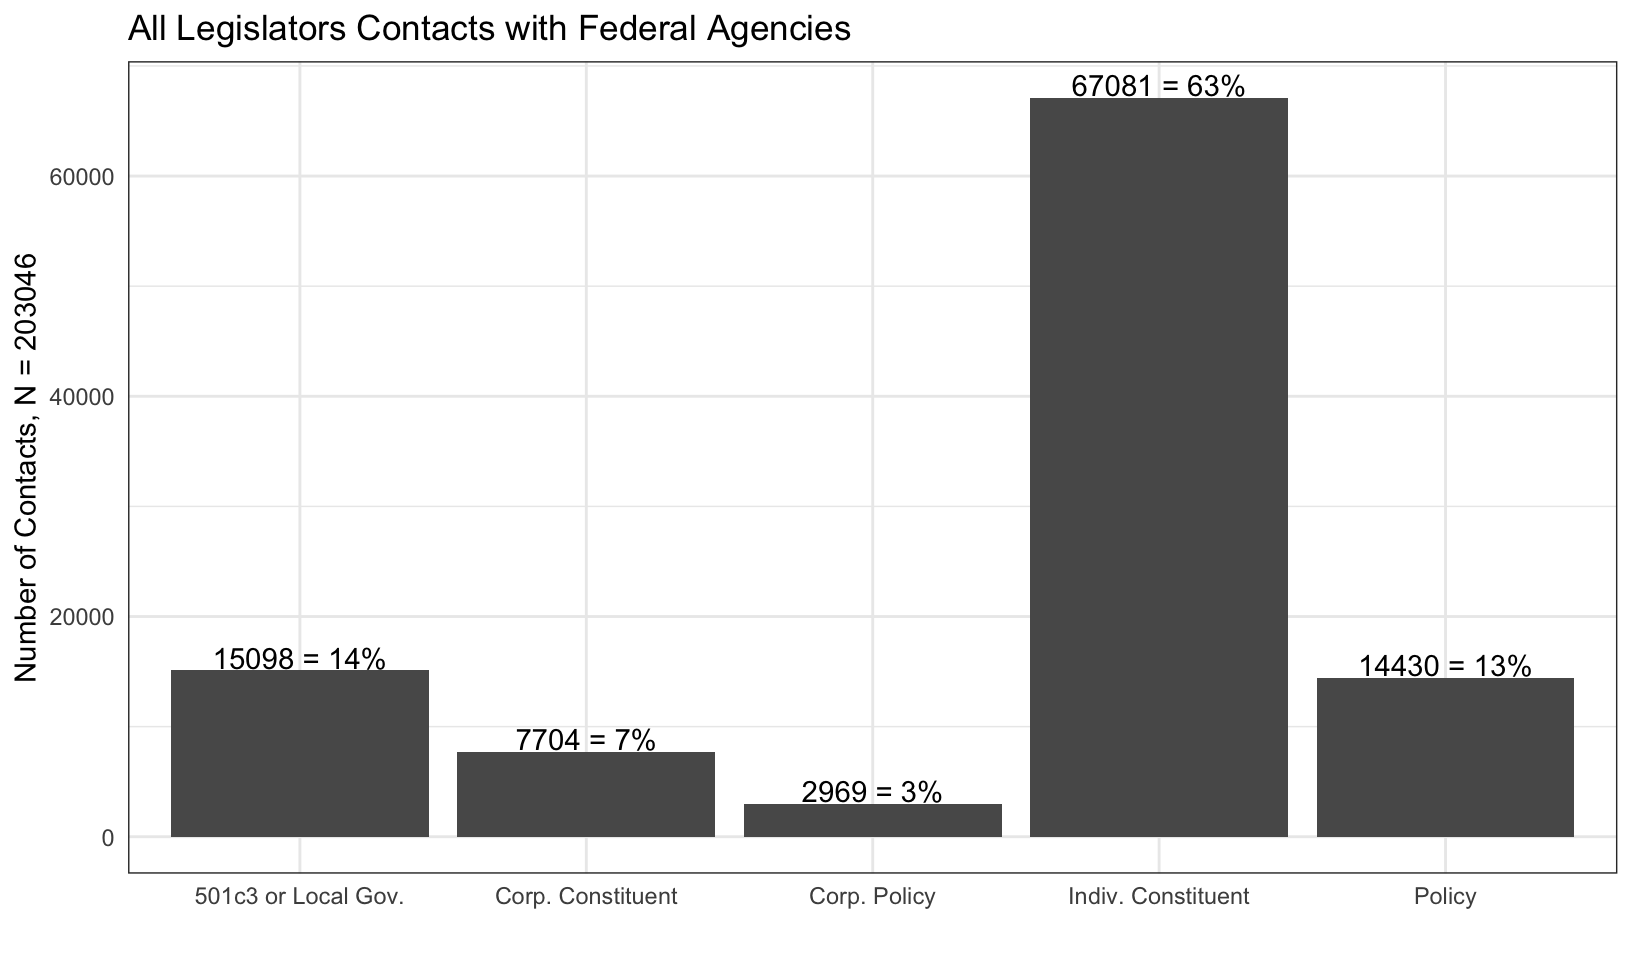
\includegraphics[width=\textwidth]{data-by-type-all-1.png}
%\end{subfigure}
\end{figure}

In contrast to the broader patterns we observe in letter-writing to all agencies, we find very different patterns of letter-writing to FERC. We observe much less individual constituent service and advocacy on behalf of local governments and non-profits, and much greater levels of corporate advocacy and policy-related work.  Notably, across all agencies, letter-writing on behalf of corporate constituents is the least common form of letter-writing activity, nearly 45\% of the letters to FERC are on behalf of individual for-profit corporations. 

We can learn more by considering not just on whose behalf the letter is written, but also what the letter is advocating for or against.  In Figure \ref{f:constituentbusiness} below, the left panel looks only at letters written on behalf of an individual constituent and shows our coding of letters into four categories: Against a named business (Antibusiness), In favor of a named business (ProBusiness), Both against and for named businesses, and Other.  It is worth noting that Other here is a catch-all category that may include advocating for or against specific regulations that may benefit (or harm) a business, but no individual business names were mentioned in the letter.  The right-hand panel breaks down letters into the same four categories but only looks at letters not written on behalf of individual constituents (i.e., all other types of letters, including those written on behalf of corporations).  

\begin{figure}[ht!]
\centering
\caption{} \label{f:constituentbusiness}

\includegraphics[width=\textwidth]{constituent-non-constituent-1.png}
\caption*{\textbf{Figure \ref{f:constituentbusiness}: What Types of Letters are Supportive of Businesses?}  The left panel shows letters written to FERC on behalf of individual constituents and the right panel shows letters written to FERC on behalf of non-constituents.  The bars show what those letters were actually arguing for substantively broken down into four categories: against a named business (Antibusiness), in favor of a named business (Probusiness), both for and against named businesses (Both), and Other (other is a catch-all category that may include advocating for or against specific regulations which may benefit (or harm) a business, but no business names were mentioned in the letter. }
\end{figure}

In sum, Figure \ref{f:constituentbusiness} provides strong evidence that most constituent letters are advocating against businesses rather than in favor of businesses.  In contrast to the constituent letters, most non-constituent letters advocate in favor of named businesses. 

\section{Which Members Attempt to Influence FERC?}

We begin our exploration of what members attempt to influence the Federal Energy Regulatory Commission by examining the legislators most active in their communications with FERC. These figures use data from 2000-2018.  Figure \ref{f:activity} below shows the most active legislators and their letter-writing activity over time (2000-2018).  The top panel shows the most active Senators, and the bottom panel shows the most active Representatives.  Each hash mark indicates the legislator wrote a letter on that date.\footnote{Readers should be aware that some of the members listed in the table weren't in the chamber for the entire period, so blank stretches at the end or beginning of the line may indicate the member was out of office during that period.}  

\begin{figure}[ht!]
\centering
\caption{}\label{f:activity}
\begin{subfigure}{\columnwidth}
%\caption{Senators Most Attempting to Influence FERC}\label{f:senatebarcode}

\includegraphics[width = \textwidth]{members_barcoded-1.png}
\end{subfigure}
\begin{subfigure}{\columnwidth}
%\caption{Representatives Most Attempting to Influence FERC}\label{f:housebarcode}

\includegraphics[width = \textwidth]{members_barcoded-2.png}
\end{subfigure}
\caption*{\textbf{Figure \ref{f:activity}: Legislators Writing the Most Letters to FERC.} The top panel shows the Senators who wrote the most letters to FERC and the bottom panel shows the Representatives who wrote the most letters to FERC.  Each hash mark indicates the legislator wrote a letter on that date. Note that many members listed in the table weren't in the chamber for the entire period, so blank stretches at the end or beginning of the line may indicate the member was out of office during that period.}
\end{figure}

As the bottom panel of Figure \ref{f:activity} shows, Rep. Virgil Goode was one of the most active House letter-writers to FERC.\footnote{Also of note is that Rep. Goode is one of the relative few party-switchers in recent congresses.  He switched from a Democrat to Independent prior to the 2000 election and then switched from Independent to Republican prior to the 2002 election.}  Interestingly, his letter-writing activity was largely focused on FERC with over 67\% of his total letters (across all agencies) written to FERC. During the period of his greatest letter-writing intensity, electric utility companies (which are overseen by FERC) were one of his greatest sources of campaign contributions. The letters Rep. Goode wrote to FERC illustrate the challenge of linking issues discussed in the letters to campaign contributions.  Rep. Goode's letters mention the Smith Mountain Project and Appalachian Power.  These are a project and subsidiary company related to the same parent company American Electric Power (also referred to as AEP).  

Letter-writing activity varies by party and majority-minority status in Figure \ref{f:party} below. The upper left-hand panel shows for the time the Democrats controlled the majority of the chamber, the percentage of letters they wrote to FERC on behalf of constituents, and the percentage advocating on behalf of businesses.  The upper right-hand panel shows the same proportions for when Republicans controlled the majority, the lower right-hand panel shows the proportions for when the Republicans were in the Minority, and the lower left-hand panel shows the proportions for when the Democrats were in the Minority.   

\begin{figure}[ht!]
\centering
\caption{} \label{f:party}

\includegraphics[width=\textwidth]{part-constituent-1.png}
\caption*{\textbf{Figure \ref{f:party}: Who Writes on Behalf of Constituents vs. Business?  By Party and Majority Status}. The upper left panel represents letters to FERC that Democrats wrote while they were in the majority, what percentage were advocating on behalf of constituents and what percentage were advocating on behalf of businesses.  The upper right panel shows the same proportions for Republicans while they were in the majority, the lower right for Republicans while they were in the minority, and the lower-left for Democrats while they were in the Minority. }
\end{figure}

In dis-aggregating letter-writing activity by party and majority status in Figure \ref{f:party}, we observe that Democrats and Republicans behave differently, and they behave differently when they're in the majority versus when they're in the minority.  When Republicans controlled the majority, they write approximately 60\% of their letters to FERC advocated on behalf of named businesses.  In contrast, when the Republicans were in the minority, those ratios flip, and they write nearly 70\% of their letters on behalf of constituents.  

We observe very different letter-writing activity for the Democrats.  When the Democrats are in the majority, they write approximately 65\% of their letters on behalf of constituents -- notably different than Republicans in the majority who were primarily advocating on behalf of companies while in the majority.  When Democrats lose majority status, their advocacy moderately changes, so that they write more than half of their letters on behalf of businesses. It is notable that while both parties change their behavior when they move from the majority to the minority, the change in behavior is substantially greater for Republicans.  

\section{Demand Driven Letter-writing?}

One of the challenges of our approach to studying legislative letter-writing to federal agencies is that we don't observe the demand for letters from constituents or businesses.  In an ideal world, we would measure and control for the demand for legislator advocacy.  However, since our project covers both the U.S. House and the U.S. Senate, we can take advantage of the large differences in state population to proxy for the demand for letter-writing from constituents.  For example, in 2018, the most populous state of California had a population of 39,557,045, while the least populated state of Wyoming had a population of only 577,737 \citep{WikipediaPop2019}.  Thus California's population is approximately 68 times that of Wyoming, and it is not unreasonable to assume that California's senators receive more requests for constituency service than Wyoming's senators.  

In our research across federal agencies, we typically see senators from larger states doing more constituency service than senators from smaller states. Figure \ref{f:statepop} below shows average Senate letter-writing by state population. The top panel Senate letter-writing to all agencies in which we observe this positive relationship between state population and Senate letter-writing to all agencies. The bottom panel shows the relationship between state population and only Senate letter-writing to FERC.\footnote{Readers should be careful in noting the differences in y-axis scales between the two panels of this figure.}  The figures include lowess smoothing trend lines and 95\% confidence intervals. 

\begin{figure}[ht!]
\centering
\caption{}\label{f:statepop}
\begin{subfigure}{0.8\textwidth}
\caption{Letters to All Agencies}

\includegraphics[width=\linewidth]{../Figs/population-1.png}
\end{subfigure}
\begin{subfigure}{0.8\textwidth}
\caption{Letters to FERC}

\includegraphics[width=\linewidth]{population-1.png}
\end{subfigure}
\caption*{\textbf{Figure \ref{f:statepop}: State population and Senate Letter-writing.}  The top panel shows average Senate letter-writing to all* agencies by state population, and the bottom panel shows the average Senate letter-writing to FERC by state population. The figures include a lowess smoothing trend line and 95\% confidence intervals. }
\end{figure}

By comparing across letter-writing to all agencies (the top panel) and letter-writing only to FERC (the bottom panel), in Figure \ref{f:statepop}, we see a weaker relationship between a state's population and letter-writing to FERC than we observed in the agency-wide data as a whole. While Figure \ref{f:statepop} shows the name and state of high-letter writing outlier Senators, it is difficult to identify the number of letters coming from each state in the figure.  To more clearly highlight what states show the highest level of senatorial letter-writing, Figure \ref{f:statepoptotal} shows the number of Senate letters to FERC by state.  The left panel shows a heat map for the total number of letters written to FERC from senators from that state, while the right panel shows a heat map for senatorial letter-writing to FERC adjusted by the state's population (per million residents).  The lighter colors show a higher intensity of senatorial letter-writing from that state.     

\begin{figure}[ht!]
\centering
\caption{}\label{f:statepoptotal}
\begin{subfigure}{0.48\textwidth}

\includegraphics[width=\linewidth]{sentate_percapita_map-1.png}
\end{subfigure}
\begin{subfigure}{0.48\textwidth}

\includegraphics[width=\linewidth]{sentate_percapita_map-2.png}
\end{subfigure}
\caption*{\textbf{Figure \ref{f:statepoptotal}: FERC Contacts from Senators by State.} The left panel shows the total number of FERC contacts from senators by state.  The right panel shows the contact per million residents from senators by state. Lighter colors show greater letter-writing activity.}
\end{figure}

As we saw in Figure \ref{f:statepop}, there is only a weak relationship between state population and senatorial letter-writing to FERC.  The left-hand panel of Figure \ref{f:statepoptotal} shows that while some senators from highly populated states write a lot of letters such as senators from California and New York, other highly populated states such as Florida barely register.  Once we adjust for state population (a rough proxy for constituent demand) and turn our attention to the right-hand panel in Figure \ref{f:statepoptotal}, we see that Senate letter-writing from California and New York no longer stands out.  

After adjusting for state population, we see that the most active letter-writing Senate delegations hail from Maine, Vermont, Wyoming, Rhode Island, and Montana.  While some of these population-adjusted state leaders may be a surprise, others seem consistent with the role the energy sector plays in each state's economy.  For example, Wyoming is per capita the top energy-producing state in the country with substantial reserves of oil and natural gas \citep{Wyoming2019}. Western state officials and their congressional delegations are also known to be particularly active on electricity grid policy, where there have recently been high-profile conflicts between state regulations and FERC regulations (personal correspondence with Ben Serrurier, Senior Manager of Market Development at an electric power developer). 

In addition to the number of people a legislator represents, some legislators' constituents may demand more attention to energy policy than others.
To address other components of demand-driven letter writing in robustness checks below, we include a measure of how important energy businesses are in legislators' districts.  While it is difficult to have a direct measure of which energy firms will have business before FERC, we use data from the American Community Service to measure the number of employees in energy-related positions within the district.\footnote{The the closest overlapping category is all workers in transportation, warehousing, and utilities.}. While this is not a direct measure of demand for FERC activity, it is a proxy of energy interest within a district. 

% \section{Congressional Committee Oversight and Letter-writing}

% Turning from constituent demand as a driver of legislator behavior to the role of their institutional position, we explore how policy-relevant committee chairs interact with FERC.  Given FERC's role in regulating the interstate transmission of electricity, natural gas, and oil, we identified two policy-relevant oversight committees in each chamber of Congress.  In the House, we examine members of the House Energy and Commerce Committee and the House Natural Resources Committee.  In the Senate, we examine members of the Senate Committee on Energy and Natural Resources and the Senate Committee on Environment and Public Works. Figure \ref{f:chairs} below shows the letter-writing activity of committee chairs of these committees both before, during, and after their time as chair.  

% \begin{figure}[ht!]
% \centering
% \caption{}\label{f:chairs}
% 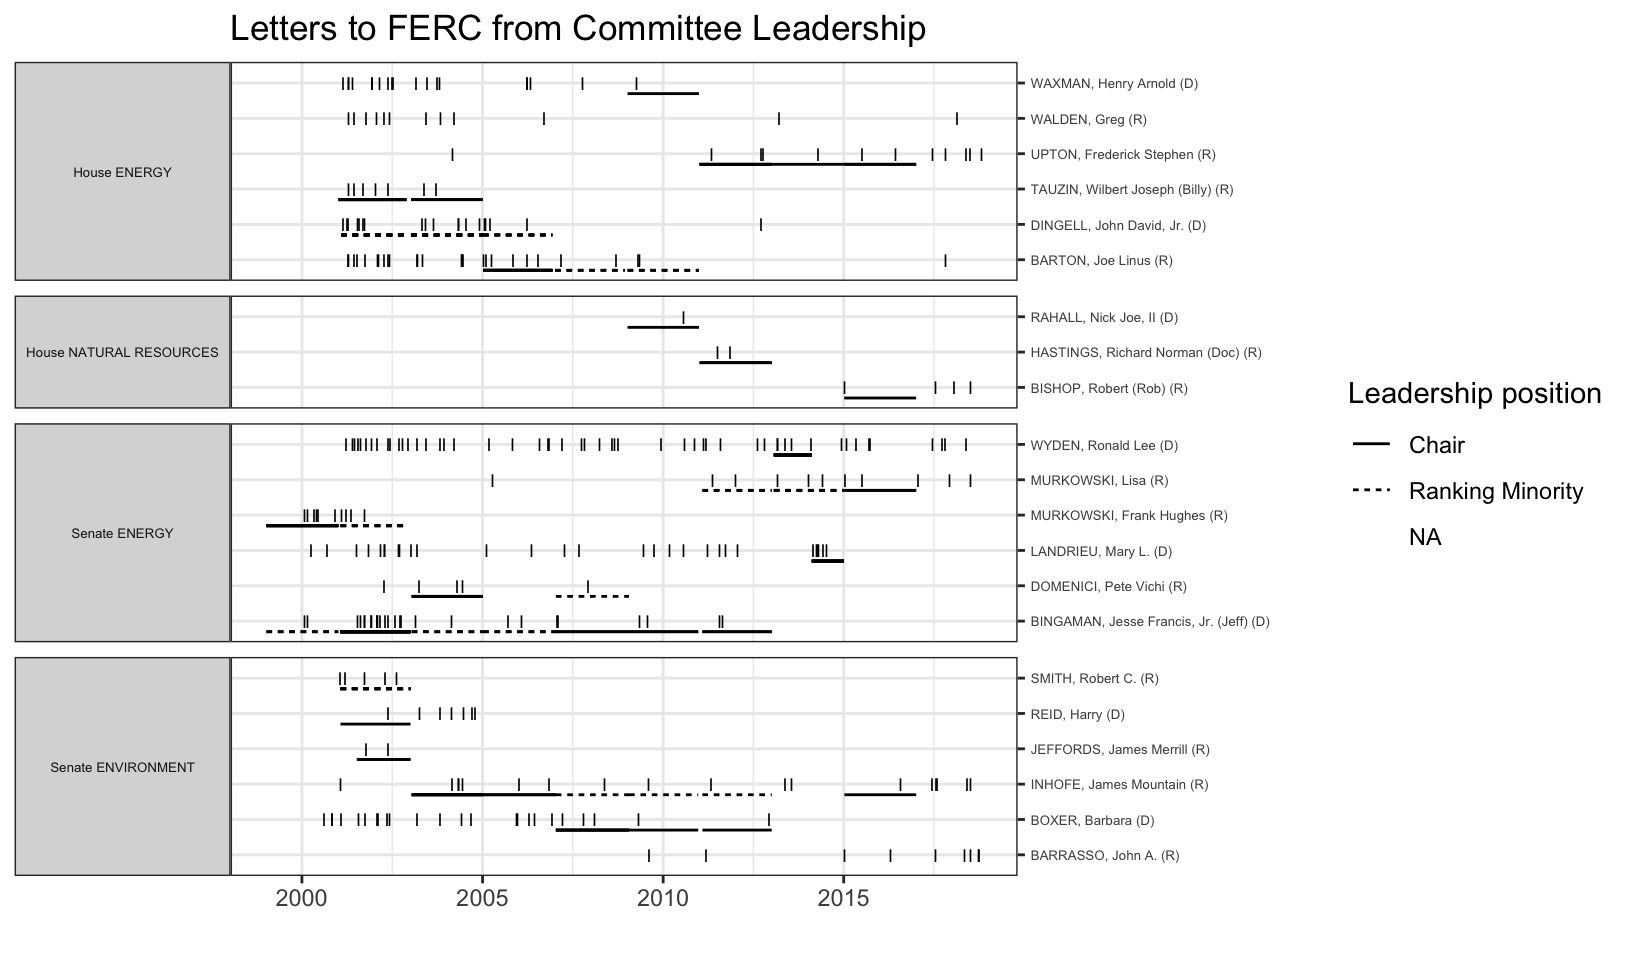
\includegraphics[width = \textwidth]{committeechiars_barcode-1.png}
% \caption*{\textbf{Figure \ref{f:chairs}: Committee Chairs Attempting to Influence FERC.} Each hash mark indicates the legislator wrote a letter on that date. The solid horizontal lines indicate the period for which that member was a committee chair; the dashed horizontal lines indicate the period for which that member was ranking member (top minority party leader) of the committee.  Note that many members listed in the table weren't in the chamber for the entire period, so blank stretches at the end or beginning of the line may indicate the member was out of office during that period.}
% \end{figure}

% Figure \ref{f:chairs} shows that committee chairs of policy-relevant committees regularly wrote letters to FERC. This is particularly true for the Energy and Commerce Committee in the House and the Senate Committee on Energy and Natural Resources, which is the more policy-relevant committee for each chamber, and whose chairs were active letter writers before, during, and after their time as chair. Letters may thus reflect ongoing relationships that legislators have in a policy area and relevant agencies in the federal bureaucracy. 

\section{The Relationship between Letter-writing and Campaign Contributions}

Taking into account demand enables us to more effectively isolate the relationship between Political Action Committee (PAC) contributions from the energy sector to a legislators campaign and the legislator's letter-writing activity to FERC.  We are focusing exclusively on campaign contributions from political action committees in the energy sector.  We use the Center for Responsive Politics' classification of PACs into industries to identify relevant PACs.  Given our focus on the Federal Energy Regulatory Commission and the jurisdiction of that Commission, we are including in our totals all political action committees that the Center for Responsive Politics classifies as linked to companies in the Oil, Gas, or Energy sector, excluding those involved in energy extraction or manufacturing (since FERC does not regulate extraction).  We create an industry-specific total of PAC contributions to a given member in an election cycle.  Collectively this covers 428 PACs in the energy sector, which we then match to their PAC contributions received by each Member of Congress.
 
Figure \ref{f:lettersmoney1} below shows the average amount a member received in each election cycle from all energy sector PAC contributions combined.
 
 \begin{figure}[ht!]
\centering
\caption{}\label{f:lettersmoney1}
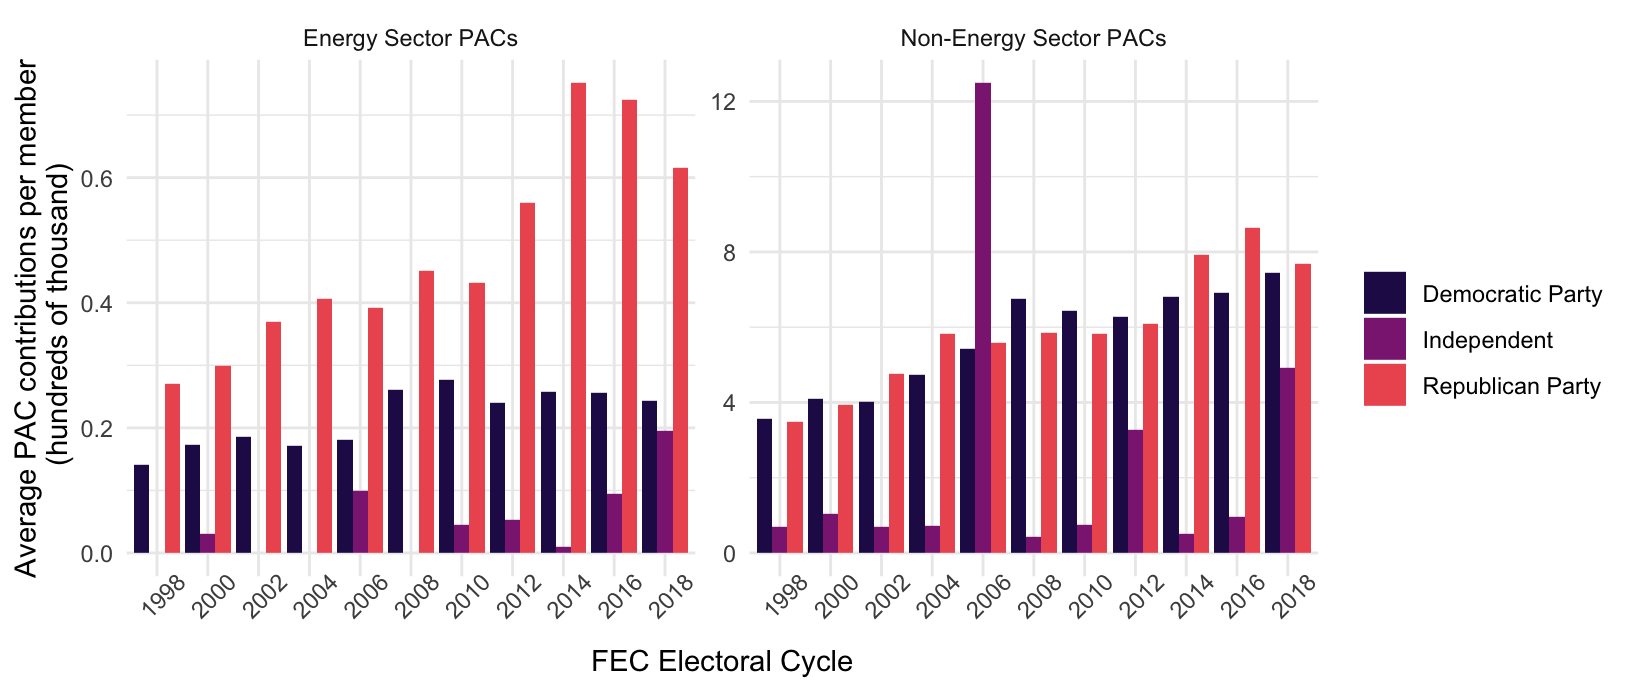
\includegraphics[width = \textwidth]{pac_amounts-2.png}
\caption*{\textbf{Figure \ref{f:lettersmoney1}: Average Energy Sector PAC Contributions Per Member Per Cycle.}}
\end{figure}

The data in Figure \ref{f:lettersmoney1} suggests that the average legislator receives considerable support for their campaigns from energy-sector PACs.  Figure \ref{f:lettersmoney2} below shows the dramatic cross-party variation in support from the energy industry.  Figure \ref{f:lettersmoney2} shows that Democrats received substantially less money from the energy sector.  For example, in the 2012 election cycle, Democrats received approximately a third of what Republicans did from the energy sector.
 
 \begin{figure}[ht!]
\centering
\caption{}\label{f:lettersmoney2}
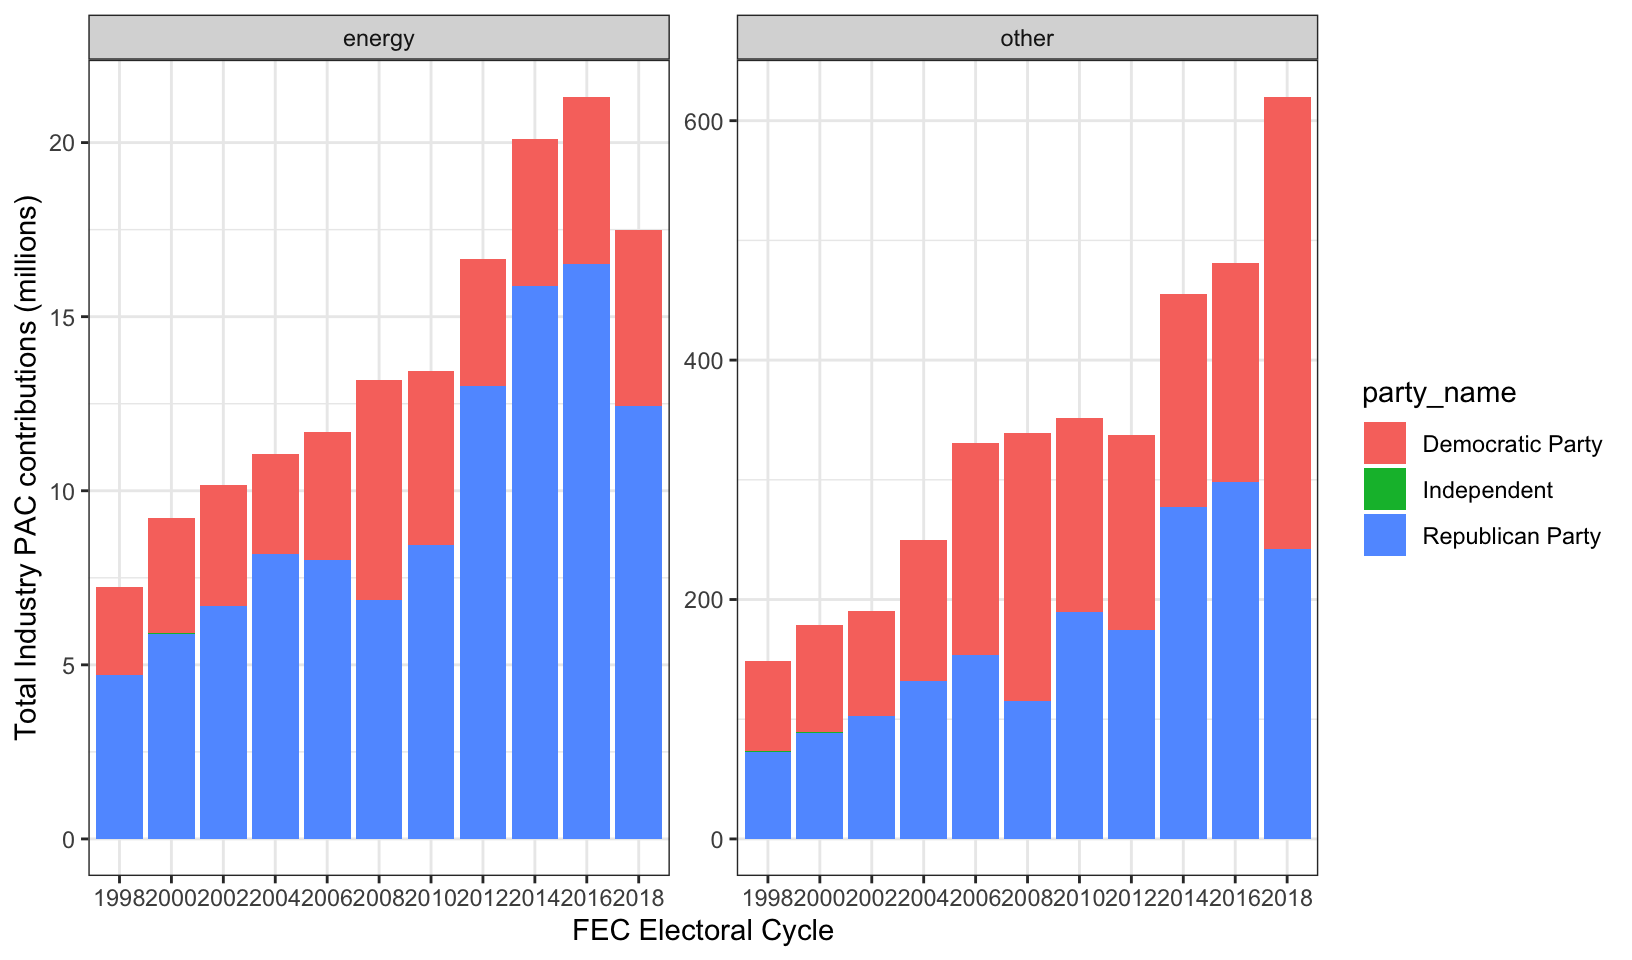
\includegraphics[width = \textwidth]{pac_amounts-1.png}
\caption*{\textbf{Figure \ref{f:lettersmoney2}: Cross-Party Differences in Campaign Contributions from Energy Sector PACs (left) and Non-energy Sector PACs (right).} Note: The y-scales differ. }
\end{figure} 

\begin{figure}[ht!]
\centering
\caption{}\label{f:pac_amounts-3}
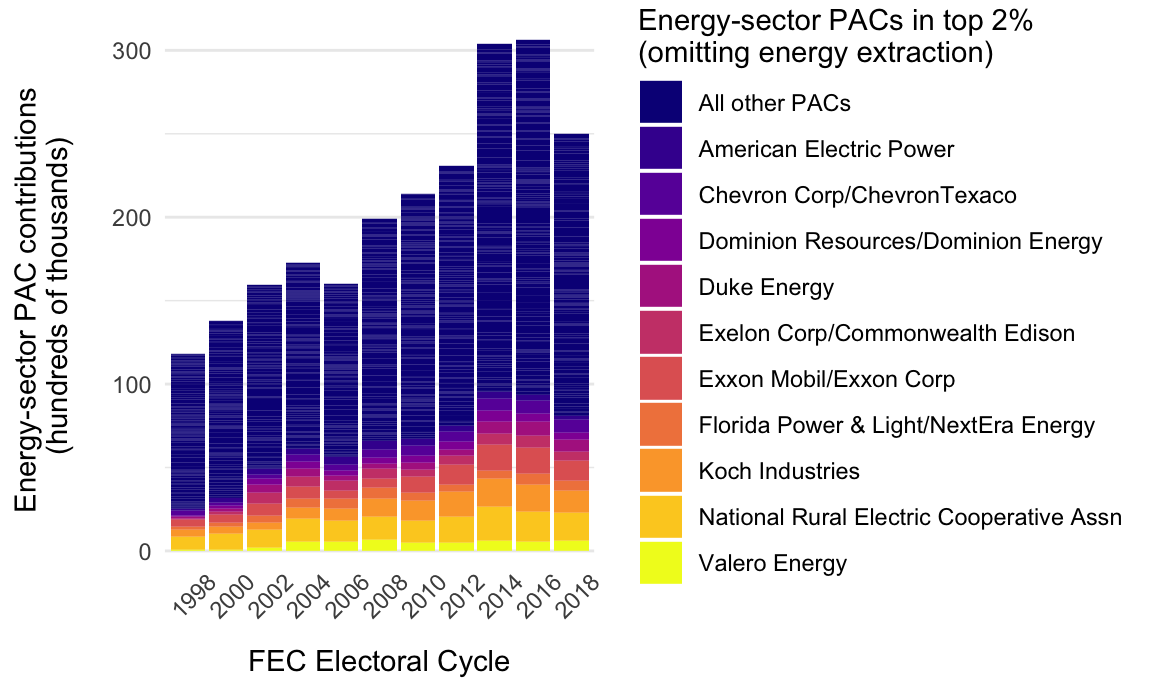
\includegraphics[width = \textwidth]{pac_amounts-3.png}
\caption*{\textbf{Figure \ref{f:pac_amounts-3}: Unequal Money Across Energy Sector PACs}. The ten PACs that comprise the top 2\% of energy PACs (omitting energy extraction) contribute a disproportionate share of the energy industry's contributions.  The contribution activity of those PACs across election cycles is highlighted in individual colors.}
\end{figure} 

We also observe substantial inequality across energy-sector PACs in how much money they contribute to congressional campaigns.  Figure \ref{f:pac_amounts-3} highlights the money that the ten PACs that comprise the top 2\% of energy PACs.  The most active energy-sector PAC in the 2012 cycle was the Bechtel Company PAC, which contributed well over half a million dollars to members of Congress in that cycle. The energy-sector PACs with the largest contributions in the 2018 cycle were the National Rural Electric Cooperative, Koch Industries, and Exxon. These differences across PACs and the often diverging goals of competing companies suggest that linking specific PACs to the companies and projects mentioned in the congressional letters to FERC may be a promising area for future research.  In the concluding section, we discuss how we plan to pursue this line of research.

Having established that energy sector political action committees spend substantial sums of money on congressional campaigns, we now ask whether member-level variation in campaign funding from the energy sector is correlated with variation in legislator's letter-writing to FERC. The dependent variable in each model is the number of letters written by a legislator in a congress, either on behalf of energy-sector businesses, opposing energy-sector businesses, on behalf of individual constituents, or all of the above (i.e., the "type" of letter). In Figure \ref{f:model1}, we see the coefficient and 95\% confidence intervals for energy industry PAC contributions on letter-writing activity to FERC.  These models are bivariate Poisson regression models in which each color represents a different dependent variable (the type of letter).\footnote{All models presented in this paper are Poisson regression since all dependent variables are counts of different types of letters.  We obtain nearly identical substantive results with OLS regression.} The full regression tables for this model are in Table \ref{tab:bimoney} in the Appendix.\footnote{Frequently, the literature on campaign contributions posits non-linear relationships, and in particular, we often see natural log transformation implying diminishing effects of money as the amount increase.  Table \ref{tab:bilogmoney} in the Appendix shows the same bivariate contribution models, but with the contribution amounts transformed using natural logs.  Table \ref{tab:bicareermoney} in the Appendix shows the same bivariate contribution models, but with the total amount of money received from the industry over a member's entire career. } 

\begin{figure}[ht!]
\centering
\caption{}\label{f:model1}
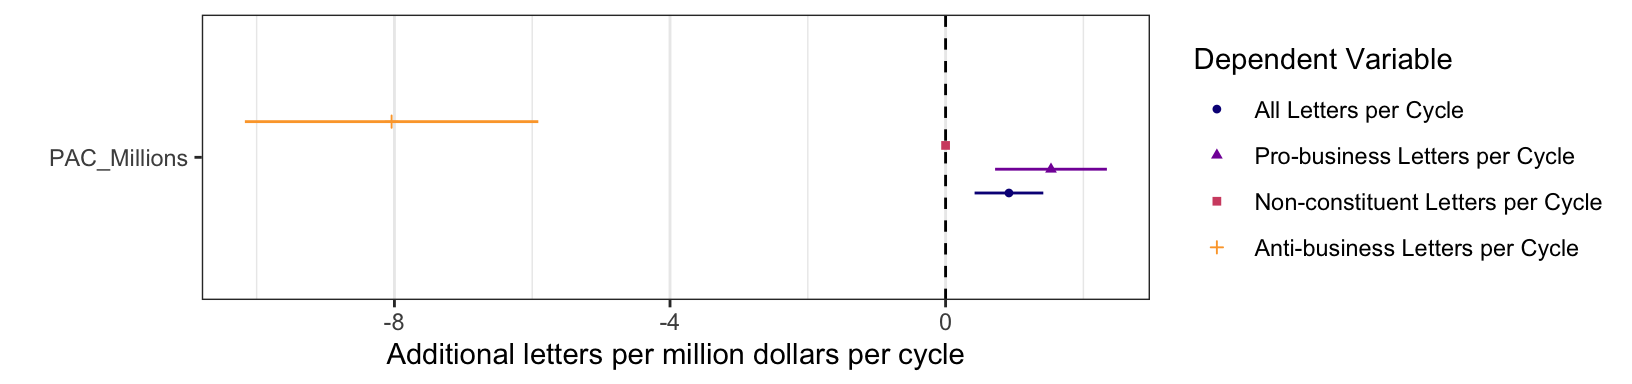
\includegraphics[width = \textwidth]{models-1.png}
\caption*{\textbf{Figure \ref{f:model1}: Bivariate Models - Campaign Contributions and Letter-writing to FERC.} These figures show the point estimate and 95\% confidence intervals for the energy industry PAC contributions on letter-writing activity to FERC.  Each color represents a different dependent variable (a different type of letter). The full regression tables for this model are in Table \ref{tab:bimoney} in the Appendix.}
\end{figure}

The bivariate campaign contribution and letter-writing regression results in Figure \ref{f:model1} show a positive relationship for overall letter-writing to FERC per cycle and Pro-Business Letter-writing to FERC per cycle. They show a somewhat weaker relationship between Anti-Business Letter-writing to FERC and no evidence of a relationship between constituent letters and campaign contributions.  In terms of the magnitude of the effect size, the model suggests that \$100,000 dollars in contributions from energy sector PACs in a cycle correlates with 0.35 additional pro-business letters written to FERC in the following congress. We obtain a nearly identical estimate when we include a measure of the number of employees in the district (0.34 letters).

%Frequently, the literature on campaign contributions posits non-linear relationships, and in particular, we often see natural log transformations implying diminishing effects of money as the amount increases.  Figure \ref{f:model2} below shows the same bivariate contribution models, but with the contribution amounts transformed using natural logs. 

%\begin{figure}[ht!]
%\centering
%\caption{}\label{f:model2}
%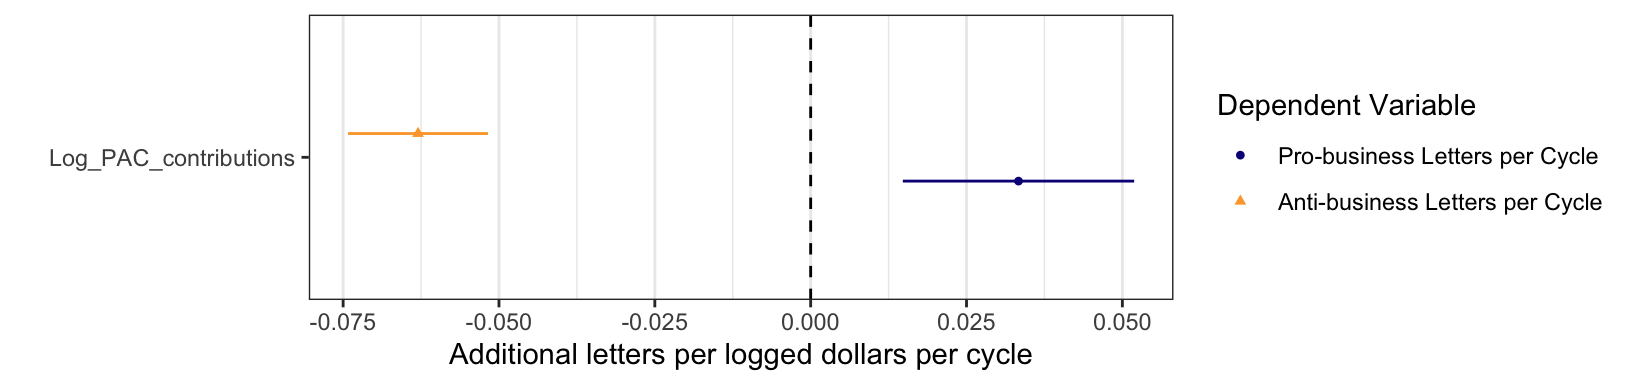
\includegraphics[width = \textwidth]{models-log-1.png}
%\caption*{\textbf{Figure \ref{f:model2}: Bivariate Models - Log Campaign Contributions and Letter-writing to FERC.} These figures show the point estimate and 95\% confidence intervals for the natural log of energy industry PAC contributions on letter-writing activity to FERC.  Each color represents a different dependent variable (type of letter).}
%\end{figure}

Turning from campaign contributions to party membership, we observed large partisan differences in letter-writing activity earlier in the paper in Figure \ref{f:party}.  In Figure \ref{f:model4} below, we see a bivariate model looking at the relationship between being a Republican and writing letters to FERC.\footnote{The full regression model is available in Table \ref{tab:biparty} in the Appendix.}  The results in Figure \ref{f:model4} show stark partisan differences in letter-writing.  We see Republicans writing significantly more pro-business letters than Democrats and writing many fewer anti-business letters than Democrats.  

\begin{figure}[ht!]
\centering
\caption{}\label{f:model4}
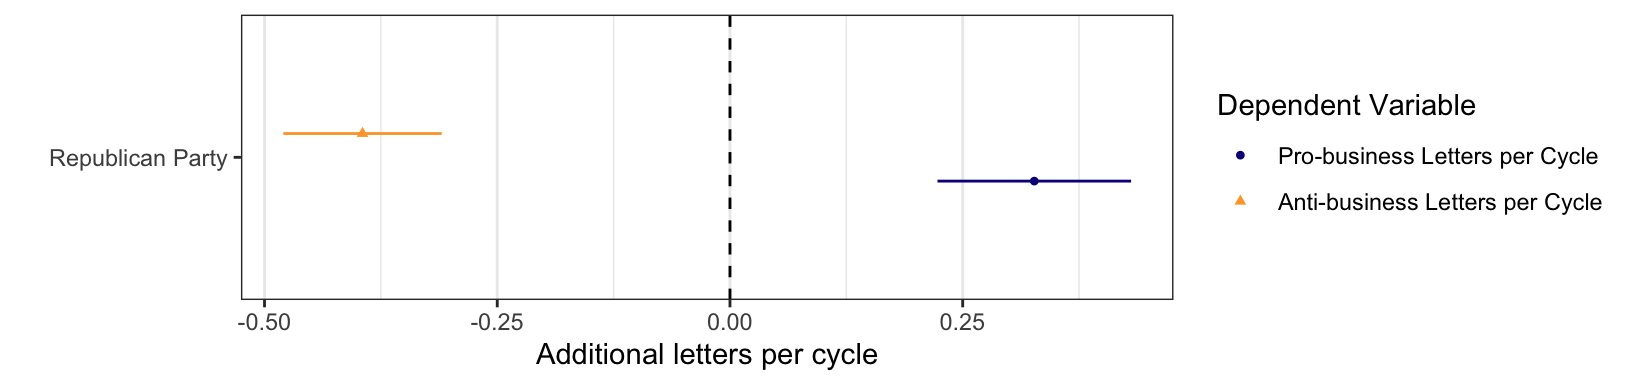
\includegraphics[width = \textwidth]{models-party-1.png}
\caption*{\textbf{Figure \ref{f:model4}: Bivariate Models - Party Membership and Letter-writing to FERC.} These figures show the point estimate and 95\% confidence intervals for being a Republican legislator on letter-writing activity to FERC.  Each color represents a different dependent variable (type of letter). The full regression model is available in Table \ref{tab:biparty} in the Appendix.}
\end{figure}


  

 
%\begin{figure}[ht!]
%\centering
%\caption{}\label{f:model3}
%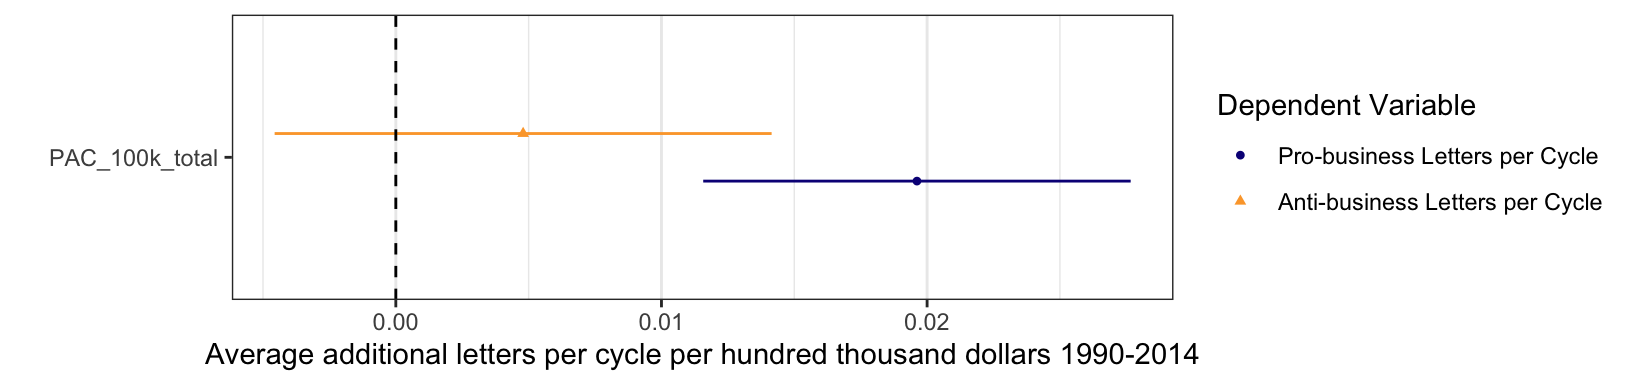
\includegraphics[width = \textwidth]{models-total-1.png}
%\caption*{\textbf{Figure \ref{f:model3}: Bi-variate Models - Career Campaign Contributions and Letter-writing to FERC.} These figures show the point estimate and 95\% confidence intervals for the member's entire career worth of energy industry PAC contributions on letter-writing activity to FERC.  Each color represents a different dependent variable (type of letter).}
%\end{figure}

Next, we bring both party membership and energy industry PAC contributions into a multivariate model predicting letter-writing activity to FERC.  Figure \ref{f:modelsfull} shows the point estimates and 95\% confidence intervals for the coefficients in the multivariate model with both party and energy industry PAC contributions.\footnote{The full regression table is available in Table \ref{tab:multmoney} in the Appendix.}  

\begin{figure}[ht!]
\centering
\caption{}\label{f:modelsfull}
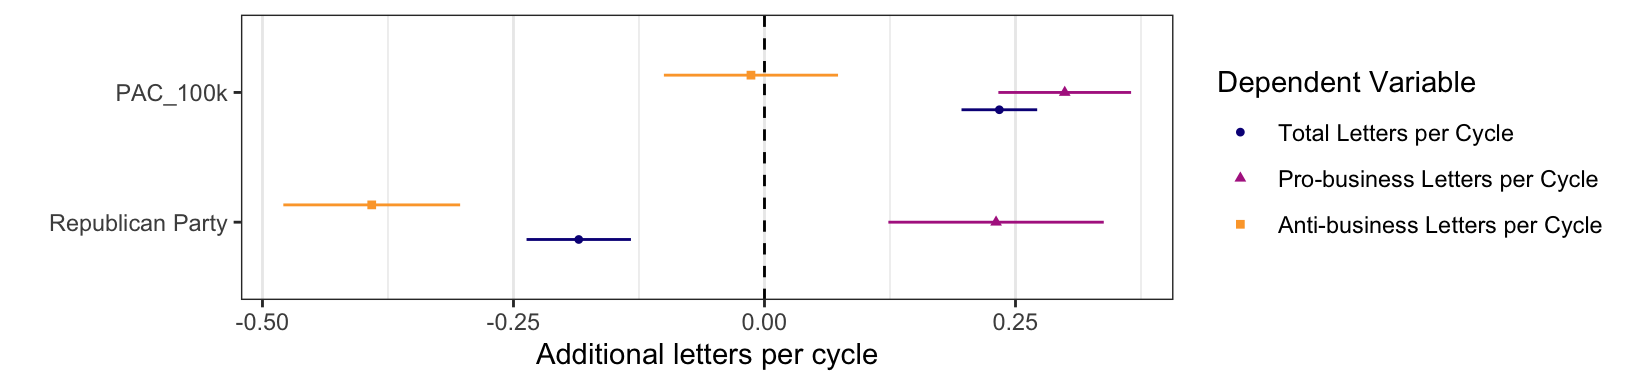
\includegraphics[width = \textwidth]{models-full-1.png}
\caption*{\textbf{Figure \ref{f:modelsfull}: Multivariate Models - Campaign Contributions, Party and Letter-writing to FERC.} These figures show the point estimate and 95\% confidence intervals for the coefficients in the multivariate model.  Each color represents a different dependent variable (type of letter).  The full regression table is available in Table \ref{tab:multmoney} in the Appendix.}
\end{figure}

By including both legislator party and energy industry campaign contributions we see in Figure \ref{f:modelsfull}, that energy industry contributions positively predict total letter-writing and pro-business letters, while they do not appear to affect anti-business letters. Again, we find that Republicans write fewer anti-business letters than Democrats.  

The findings in this section are important and provide new insights into the relationship between elected officials and PACs.  Our results demonstrate that there is a strong correlation between PAC's donations and the behavior of legislators.  But our results are slightly stronger because we account for at least one way that demand could confound our findings. Using employment in utilities within the district at least partially addresses concerns that this relationship is merely because they are legislators who focus on energy in the district. Of course, our results cannot demonstrate that there is a quid pro quo between legislators and PACs.  Rather, our evidence shows that there are relationships between legislators and PACs. Legislators receive donations from PACs, and these same legislators advocate for companies at FERC.       

\section{Conclusion}

Building on \citet{Arnold1979}'s insights into how bureaucrats and legislators \emph{anticipate} how others will react to their actions, we explored a new form of signaling and learning by examining congressional letters to the Federal Energy Regulatory Commission.  We see evidence consistent with the idea that energy industry campaign contributions lead to more over-all letters to FERC, and specifically, more pro-business letters to FERC.  

We believe this paper represents a starting point for what we can learn about legislator motivations and the impact of money on congressional and bureaucratic relations.  In future work, we hope to expand our analysis to other agencies, but also other forms of campaign contributions (super PACs, independent expenditures, lobbying data, etc.).  We also hope to look at the impact of the legislator's letters on the actions taken by the agency---in particular, we hope to focus on the speed of the review by FERC as an outcome, as this is often what companies seek in these requests. 

Finally, we think one of the most promising areas of future research is connecting company-specific campaign contributions to FERC letters. On the surface, it would seem that it would be relatively straight-forward to link political action committees associated with individual companies to the companies that legislators mention in letters to FERC. The Federal Election Commission's rules require that the PAC's name include the full name of the connected organization (sponsoring company or organization) must appear in the name of the SSF. However, one challenge in this industry area is that if a linked organization has parent companies or subsidiaries, those names may not be included in the name of the PAC. Thus we need to connect the companies to their subsidiary/parent companies.  Furthermore, the letters to FERC often only mention the name of an Energy Project that is being developed by a company and do not always include the full sponsoring company in the letter.  So to be complete, we need to link parent companies, subsidiary companies, and related energy projects.  

As an example of the challenge of connecting corporate PACs to companies and projects mentioned in FERC letters, consider the Williams Company. The Williams Company is a Fortune 500 energy company based in Tulsa, Oklahoma, whose primary business is natural gas, but also has subsidiary parts that cover petroleum and electricity generation \citep{BloombergWilliams2019}.  The Williams Company PAC has been an active contributor to congressional campaigns in recent cycles.  In the 2016 election cycle, the Williams Company PAC contributed \$392,000 to congressional candidates with 7\% going to Democrats and 93\% to Republicans.  

Connecting these contributions to letters written by members of Congress on behalf of the company is more challenging.  The Williams Company also owns the Transcontinental Pipeline Company, the Transcontinental Gas Company, and the Transco Pipeline Company.  Furthermore, they're the company behind a large number of projects such as the Atlantic Sunrise Project, and the Northeast Supply Enhancement (NESE) Pipeline, among many others. Unfortunately, for our purposes here, the name Williams doesn't appear in their subsidiary companies.  Nor does the name Williams appear in the energy projects undertaken by the company. To attempt to link parent companies that have corporate PACs that make campaign contributions like the Williams Company to the projects and subsidiary companies mentioned in the letters, we plan to draw on a combination of news reports and company filings with the Securities Exchange Commission. %While we will present some preliminary results here based on these linkages, we do not yet believe we have comprehensive coverage of these relationships.  

While the projects we have outlined here comprise an ambitious research agenda, we believe they represent a collection of concrete steps that will help advance our knowledge in this area.  Moreover, we believe that taken together, we can use them to build on the foundational insights of \citet{Arnold1979} to better understand the strategic anticipation and signaling that takes place between legislators and bureaucrats. 


\newpage
\bibliographystyle{chicago-apsr}
%\bibliography{../congress2018.bib}
\bibliography{congress2018.bib}
\newpage
\appendix 

\renewcommand{\thefigure}{A\arabic{figure}}
\setcounter{figure}{0}
\renewcommand{\thetable}{A\arabic{table}}
\setcounter{table}{0}
\section{Sample Letters to the Federal Energy Regulatory Commission}

\begin{figure}[ht!]
\centering
\caption{} \label{f:exampleconstituencyservice}
\scalebox{0.65}{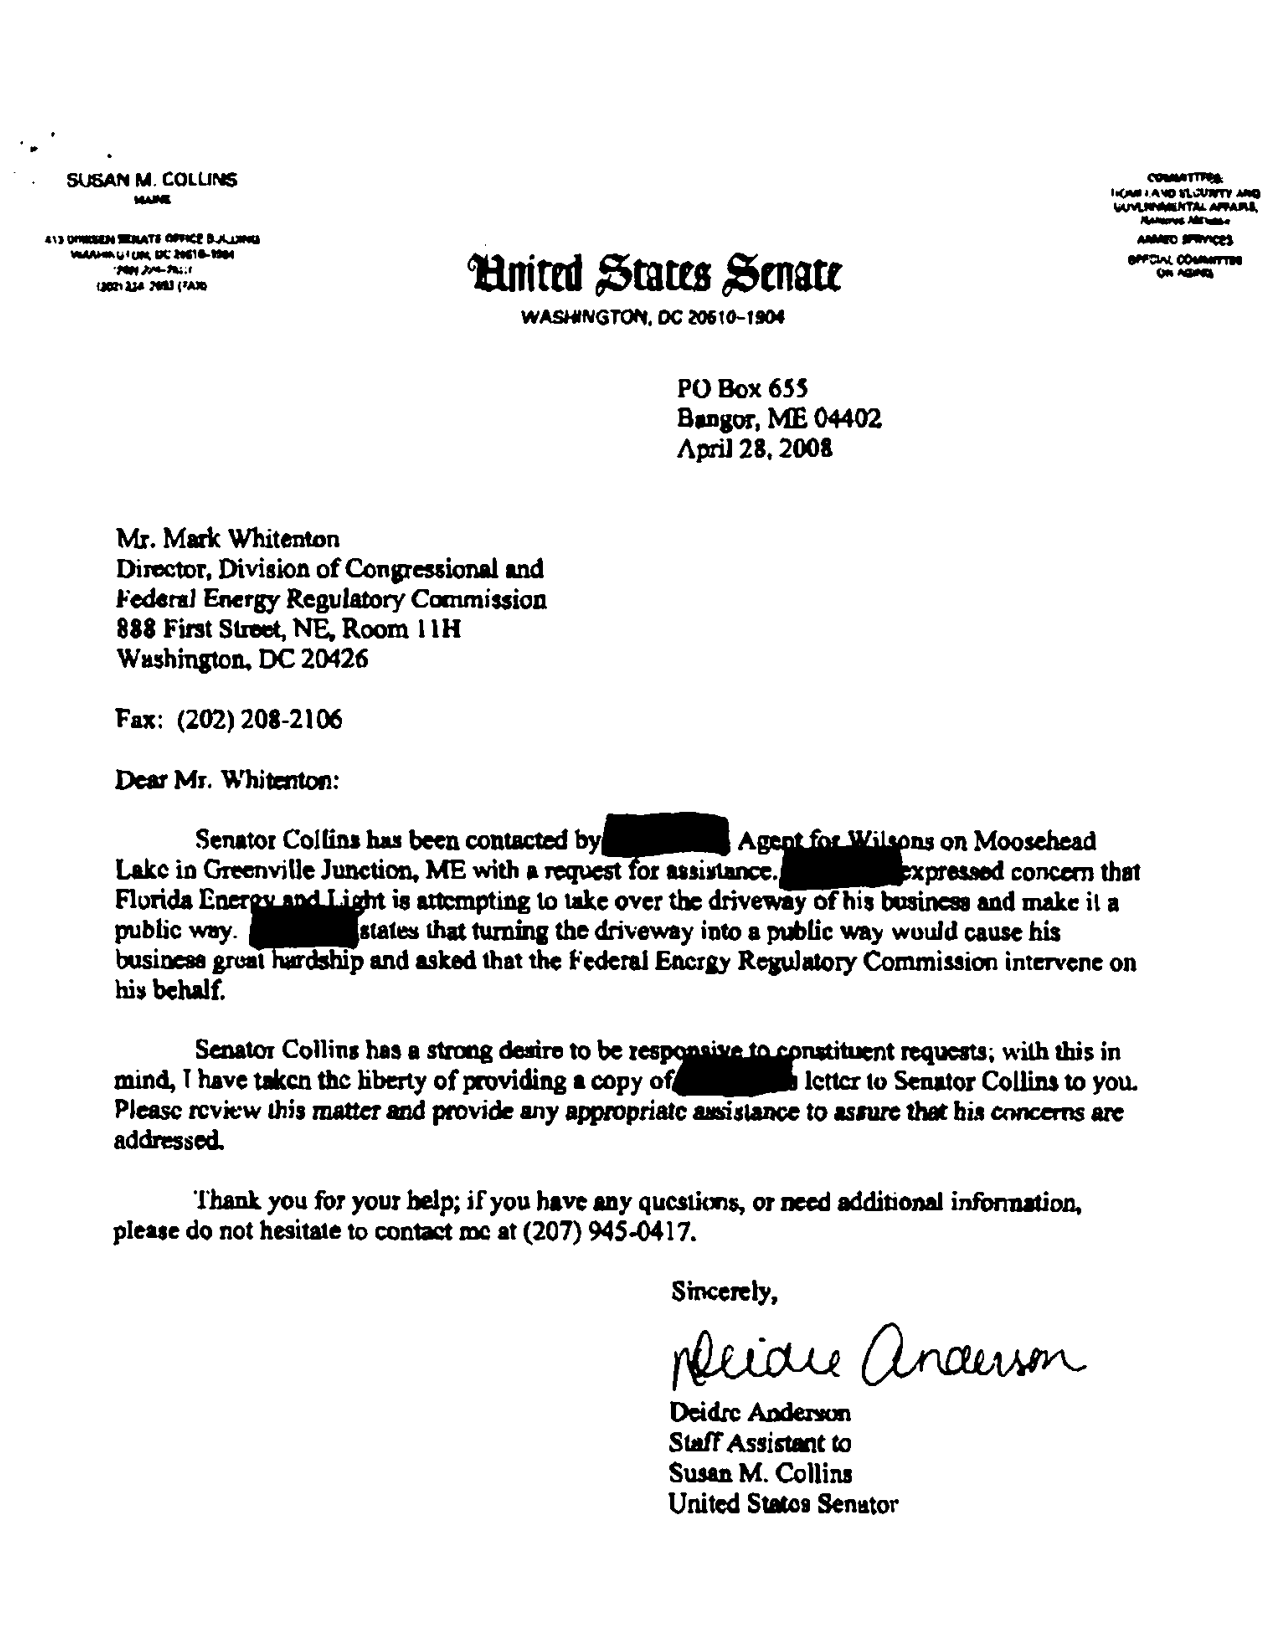
\includegraphics{20080515-0185small}}
\caption*{\textbf{Figure \ref{f:exampleconstituencyservice}: Example of Constituency Service Letter.} This is a constituency service letter written by Senator Susan Collins (R-ME) to FERC on April 28, 2008.} 
\end{figure}


\begin{figure}[ht!]
\centering
\caption{} \label{f:exampleenergyproj}
\scalebox{0.7}{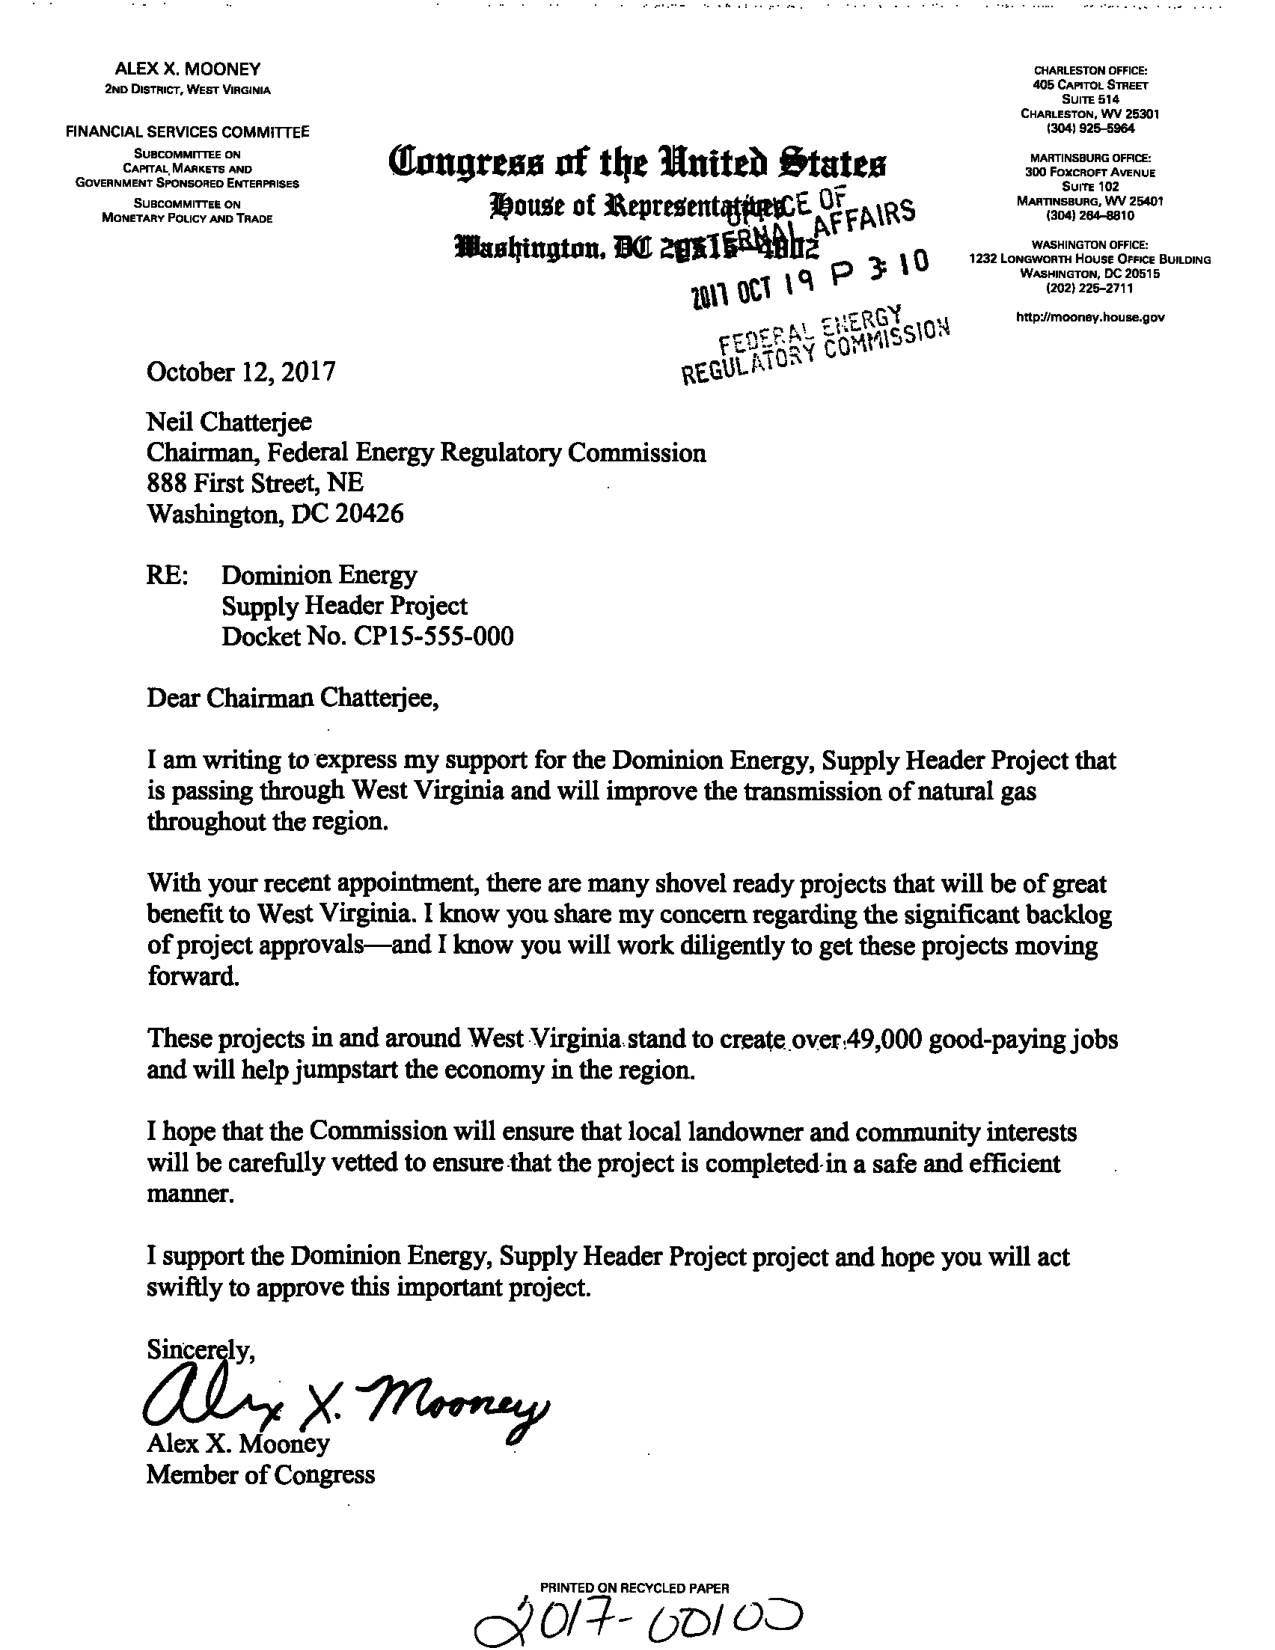
\includegraphics{20171020-0018-14718216}}
\caption*{\textbf{Figure \ref{f:exampleenergyproj}: Example of Energy Project Advocacy}. This is a letter written by Rep. Alex Mooney (R-WV2) to FERC on October 12, 2017.} 
\end{figure}

 
\begin{figure}[ht!]
\centering
\caption{} \label{f:examplepersonalbus}
\scalebox{0.8}{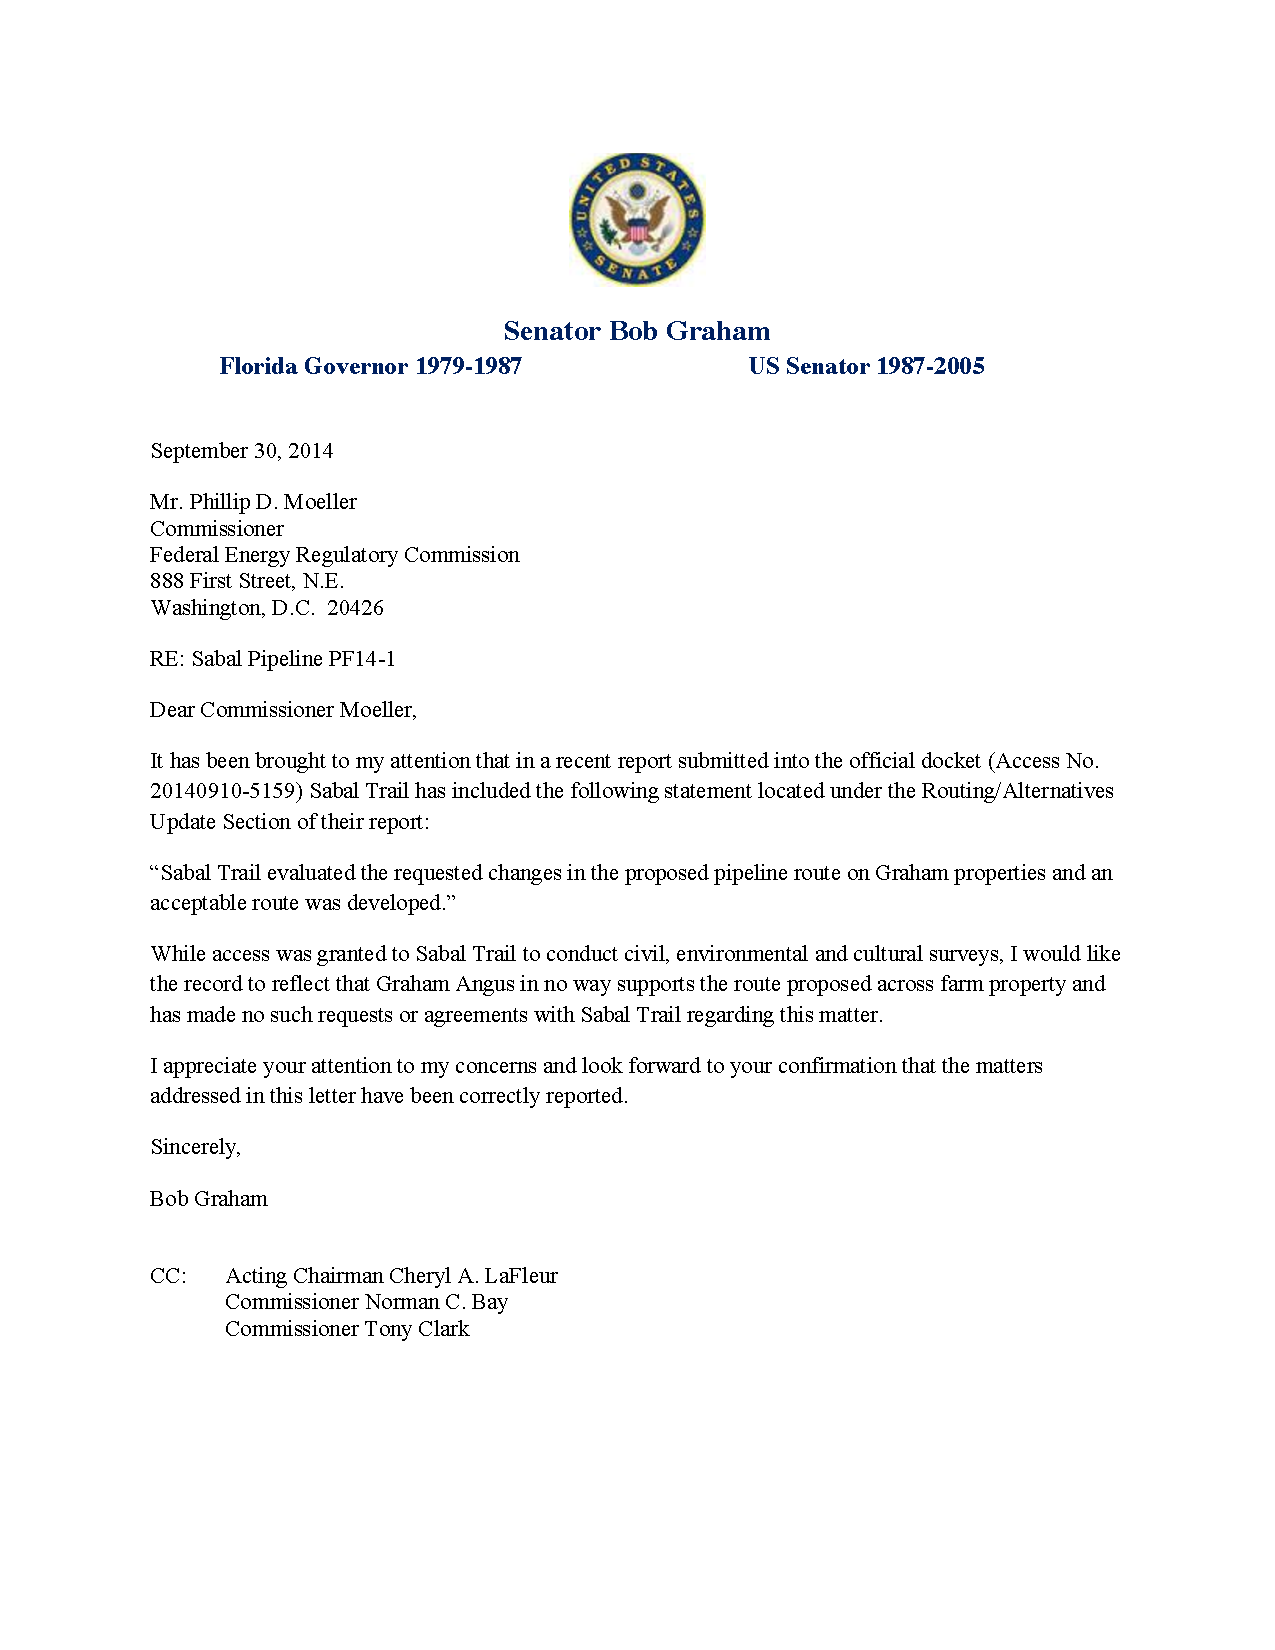
\includegraphics{20141002-4001-13649830small.pdf}}
\caption*{\textbf{Figure \ref{f:examplepersonalbus}: Example of Personal Business Interest}.  This is a letter written by former Senator Bob Graham (R-FL) to FERC on September 30, 2014. nearly a decade after retiring from the U.S. Senate.} 
\end{figure}


\section{Examples of FERC Letters}\label{a:FERC}

%The Federal Energy Regulatory Commission is one of the less well known federal agencies.  
To give readers a sense of the activities FERC regulations and the types of issues raised in congressional letters to the agency, this section presents a selection of examples.

\subsubsection{Example of Energy Project Advocacy}

As we explore in detail below, many legislator letters to FERC advocate on behalf of an energy project or another corporate interest. 
In recent years, one of the legislators most focused on advocating for energy-related projects was Rep. Alex Mooney (R-WV).  
Rep. Mooney was elected to Congress in 2014 and since that time has spent considerable time advocating for energy projects in West Virginia. In the lead-up to the 2016 congressional elections, the Charleston Gazette-Mail wrote an article highlighting the money he had received from energy companies and the approvals those companies were seeking from FERC for various projects under consideration.  They wrote, ``Dominion is trying to get the Atlantic Coast Pipeline, which would run through national forests in West Virginia, approved by the Federal Energy Regulatory Commission. Columbia Pipeline Group is hoping to have three interstate pipeline projects of its own approved by the same federal agency,''\citep[pg.4]{Brown2016cgm}.  Indeed, our data show that Mooney wrote to FERC more than any other agency, always on behalf of energy projects, mostly pipelines. 

In 2015 Rep. Mooney wrote on behalf of Columbia's Mountaineer XPress Project and Atlantic Coast Pipeline ACP project.  In 2017, he wrote on behalf of the Dominion Energy Supply Header Project, National Fuel Gas Distribution Corporation’s Northern Access Project, Transcontinental Gas Pipe Line Company's Atlantic Sunrise Project, Columbia Gas Transmission's proposed Eastern Panhandle Expansion Project, Columbia's WB Xpress Project to build new compressor stations. In addition to the tens of thousands of dollars these companies spent on Mooney's campaign, the parent companies of these projects spend millions of dollars on lobbying \citep{Lobbyview2019}.

Figure \ref{f:exampleenergyproj} in the Appendix shows one of the letters written by Rep. Mooney advocating for energy projects.  In this case, the letter clearly connects both the name of the project and the name of the company involved with the project.  Many letters lack that linkage and list only the project name, leaving us to draw those linkages.  Later in the paper, we'll discuss how we make those connections across projects, subsidiary companies, and parent companies.  


\subsubsection{Example of Constituent Service Letter}

Another frequently seen type of legislator advocacy to FERC is a constituency service letter--a letter in which the member advocates on behalf of a constituent.  Figure \ref{f:exampleconstituencyservice} in the Appendix shows an example of this type of letter. 
In this case, we observe Senator Susan Collins (R-ME) advocating on behalf of a constituent who is concerned that Florida Energy and Light is ``attempting to take over the driveway of his business and make it a public way.'' \footnote{Certain passages of this constituency service letter in Figure \ref{f:exampleconstituencyservice} have been blacked out. In this case, as we frequently observe in these letters, the constituent's name and personal information have been redacted for privacy reasons}. 


\subsubsection{Example of Personal Business Interest}

In some cases, legislators appeared motivated by personal business concerns.  For example, in 2014 former Florida Senator and Governor Bob Graham wrote to FERC regarding an issue that affected his family's farming business.\footnote{See  \url{http://miamilakes.com/AboutGraham/Overview.aspx} for a discussion of Senator Graham's relationship to the farm in question.}  The full text of this letter is in Figure \ref{f:examplepersonalbus} in the Appendix.


\clearpage
\section{Regression Result Tables}

\begin{table}[ht!]
    \centering
  

% Table created by stargazer v.5.2.2 by Marek Hlavac, Harvard University. E-mail: hlavac at fas.harvard.edu
% Date and time: Tue, Jan 21, 2020 - 20:22:37
\begin{tabular}{@{\extracolsep{5pt}}lcccc} 
\\[-1.8ex]\hline 
\hline \\[-1.8ex] 
 & \multicolumn{4}{c}{\textit{Dependent variable:}} \\ 
\cline{2-5} 
\\[-1.8ex] & total\_letters & ProBusiness\_Letters & AntiBusiness\_Letters & Constituent\_Letters \\ 
\\[-1.8ex] & (1) & (2) & (3) & (4)\\ 
\hline \\[-1.8ex] 
 PAC\_100k & 0.197$^{***}$ & 0.332$^{***}$ & $-$0.114$^{**}$ & 0.058 \\ 
  & (0.019) & (0.032) & (0.045) & (0.046) \\ 
  & & & & \\ 
 Constant & $-$0.056$^{***}$ & $-$1.540$^{***}$ & $-$0.970$^{***}$ & $-$1.438$^{***}$ \\ 
  & (0.015) & (0.030) & (0.026) & (0.031) \\ 
  & & & & \\ 
\hline \\[-1.8ex] 
Observations & 6,019 & 6,019 & 5,997 & 6,019 \\ 
Log Likelihood & $-$11,832.820 & $-$4,105.200 & $-$5,968.765 & $-$4,585.600 \\ 
Akaike Inf. Crit. & 23,669.630 & 8,214.400 & 11,941.530 & 9,175.201 \\ 
\hline 
\hline \\[-1.8ex] 
\textit{Note:}  & \multicolumn{4}{r}{$^{*}$p$<$0.1; $^{**}$p$<$0.05; $^{***}$p$<$0.01} \\ 
\end{tabular} 

  \caption{\textbf{Table \ref{tab:bimoney}: Bivariate Models - Campaign Contributions and Letter-writing to FERC}. Bivariate Poisson Regression models predicting letter-writing activity to FERC using campaign contributions from the energy industry.}\label{tab:bimoney}
\end{table}

\begin{table}[ht!]
    \centering

% Table created by stargazer v.5.2.2 by Marek Hlavac, Harvard University. E-mail: hlavac at fas.harvard.edu
% Date and time: Tue, Jan 14, 2020 - 15:03:33
\begin{tabular}{@{\extracolsep{5pt}}lcc} 
\\[-1.8ex]\hline 
\hline \\[-1.8ex] 
 & \multicolumn{2}{c}{\textit{Dependent variable:}} \\ 
\cline{2-3} 
\\[-1.8ex] & ProBusiness\_Letters & AntiBusiness\_Letters \\ 
\\[-1.8ex] & (1) & (2)\\ 
\hline \\[-1.8ex] 
 party\_nameRepublican Party & 0.327$^{***}$ & $-$0.418$^{***}$ \\ 
  & (0.053) & (0.043) \\ 
  & & \\ 
 Constant & $-$1.583$^{***}$ & $-$0.775$^{***}$ \\ 
  & (0.041) & (0.028) \\ 
  & & \\ 
\hline \\[-1.8ex] 
Observations & 5,979 & 5,744 \\ 
Log Likelihood & $-$4,101.276 & $-$5,818.336 \\ 
Akaike Inf. Crit. & 8,206.552 & 11,640.670 \\ 
\hline 
\hline \\[-1.8ex] 
\textit{Note:}  & \multicolumn{2}{r}{$^{*}$p$<$0.1; $^{**}$p$<$0.05; $^{***}$p$<$0.01} \\ 
\end{tabular} 

  \caption{\textbf{Table \ref{tab:biparty}: Bivariate Models - Party and Letter-writing to FERC}. Bivariate Poisson Regression models predicting letter-writing activity to FERC using Legislator's Party.}\label{tab:biparty}
\end{table}

\begin{table}[ht!]
    \centering
    
% Table created by stargazer v.5.2.2 by Marek Hlavac, Harvard University. E-mail: hlavac at fas.harvard.edu
% Date and time: Tue, Jan 07, 2020 - 14:24:30
\begin{tabular}{@{\extracolsep{5pt}}lcc} 
\\[-1.8ex]\hline 
\hline \\[-1.8ex] 
 & \multicolumn{2}{c}{\textit{Dependent variable:}} \\ 
\cline{2-3} 
\\[-1.8ex] & ProBusiness\_Letters & AntiBusiness\_Letters \\ 
\\[-1.8ex] & (1) & (2)\\ 
\hline \\[-1.8ex] 
 Log\_PAC\_contributions & $-$0.007 & $-$0.044$^{***}$ \\ 
  & (0.010) & (0.008) \\ 
  & & \\ 
 Constant & $-$1.868$^{***}$ & $-$1.078$^{***}$ \\ 
  & (0.094) & (0.073) \\ 
  & & \\ 
\hline \\[-1.8ex] 
Observations & 4,870 & 4,617 \\ 
Log Likelihood & $-$2,362.600 & $-$3,325.450 \\ 
Akaike Inf. Crit. & 4,729.200 & 6,654.900 \\ 
\hline 
\hline \\[-1.8ex] 
\textit{Note:}  & \multicolumn{2}{r}{$^{*}$p$<$0.1; $^{**}$p$<$0.05; $^{***}$p$<$0.01} \\ 
\end{tabular} 

  \caption{\textbf{Table \ref{tab:bilogmoney}: Bivariate Models - Logged Campaign Contributions and Letter-writing to FERC}. Bivariate Poisson Regression models predicting letter-writing activity to FERC using Logged Energy Industry Campaign Contributions.}\label{tab:bilogmoney}
\end{table}



\begin{table}[ht!]
    \centering
 
% Table created by stargazer v.5.2.2 by Marek Hlavac, Harvard University. E-mail: hlavac at fas.harvard.edu
% Date and time: Tue, Jan 21, 2020 - 19:22:24
\begin{tabular}{@{\extracolsep{5pt}}lcc} 
\\[-1.8ex]\hline 
\hline \\[-1.8ex] 
 & \multicolumn{2}{c}{\textit{Dependent variable:}} \\ 
\cline{2-3} 
\\[-1.8ex] & ProBusiness\_Letters\_Per\_Cycle & AntiBusiness\_Letters\_Per\_Cycle \\ 
\\[-1.8ex] & (1) & (2)\\ 
\hline \\[-1.8ex] 
 PAC\_100k\_total & 0.015$^{***}$ & $-$0.004$^{**}$ \\ 
  & (0.002) & (0.002) \\ 
  & & \\ 
 Constant & $-$1.567$^{***}$ & $-$0.972$^{***}$ \\ 
  & (0.033) & (0.027) \\ 
  & & \\ 
\hline \\[-1.8ex] 
Observations & 5,979 & 5,979 \\ 
Log Likelihood & $-$Inf.000 & $-$Inf.000 \\ 
Akaike Inf. Crit. & Inf.000 & Inf.000 \\ 
\hline 
\hline \\[-1.8ex] 
\textit{Note:}  & \multicolumn{2}{r}{$^{*}$p$<$0.1; $^{**}$p$<$0.05; $^{***}$p$<$0.01} \\ 
\end{tabular} 

  \caption{\textbf{Table \ref{tab:bicareermoney}: Career Bivariate Models - Campaign Contributions and Letter-writing to FERC over a Member's Entire Career}. Bivariate Poisson Regression models predicting letter-writing activity to FERC using Energy Industry Campaign Contributions.}\label{tab:bicareermoney}
\end{table}

%\begin{sidewaystable}[ht!]
%    \centering
%
% Table created by stargazer v.5.2.2 by Marek Hlavac, Harvard University. E-mail: hlavac at fas.harvard.edu
% Date and time: Thu, May 09, 2019 - 11:45:25
\begin{table}[!htbp] \centering 
  \caption{} 
  \label{} 
\begin{tabular}{@{\extracolsep{5pt}}lcccccccccc} 
\\[-1.8ex]\hline 
\hline \\[-1.8ex] 
 & \multicolumn{10}{c}{\textit{Dependent variable:}} \\ 
\cline{2-11} 
\\[-1.8ex] & All\_Letters & ProBusiness\_Letters & AntiBusiness\_Letters & Non\_Constituent\_Letters & ProBusiness\_Letters & AntiBusiness\_Letters & ProBusiness\_Letters & ProBusiness\_Letters\_Per\_Cycle & AntiBusiness\_Letters\_Per\_Cycle & AntiBusiness\_Letters \\ 
\\[-1.8ex] & (1) & (2) & (3) & (4) & (5) & (6) & (7) & (8) & (9) & (10)\\ 
\hline \\[-1.8ex] 
 PAC\_contributions & 4.238$^{***}$ & 3.786$^{***}$ & 2.102$^{***}$ & 0.00000$^{***}$ &  &  &  & 1.139$^{***}$ & 0.734$^{***}$ &  \\ 
  & (0.248) & (0.546) & (0.502) & (0.00000) &  &  &  & (0.222) & (0.218) &  \\ 
  & & & & & & & & & & \\ 
 Log\_PAC\_contributions &  &  &  &  & 0.102$^{***}$ & 0.044$^{***}$ &  &  &  &  \\ 
  &  &  &  &  & (0.011) & (0.007) &  &  &  &  \\ 
  & & & & & & & & & & \\ 
 party(R) &  &  &  &  &  &  & 0.132$^{**}$ &  &  & $-$0.256$^{***}$ \\ 
  &  &  &  &  &  &  & (0.062) &  &  & (0.048) \\ 
  & & & & & & & & & & \\ 
 Constant & $-$0.251$^{***}$ & $-$1.708$^{***}$ & $-$1.137$^{***}$ & $-$0.251$^{***}$ & $-$2.466$^{***}$ & $-$1.434$^{***}$ & $-$1.332$^{***}$ & $-$2.010$^{***}$ & $-$1.421$^{***}$ & $-$0.632$^{***}$ \\ 
  & (0.017) & (0.036) & (0.028) & (0.017) & (0.100) & (0.062) & (0.045) & (0.101) & (0.081) & (0.031) \\ 
  & & & & & & & & & & \\ 
\hline \\[-1.8ex] 
Observations & 5,170 & 5,170 & 5,170 & 5,170 & 5,170 & 5,170 & 3,712 & 899 & 893 & 3,712 \\ 
Log Likelihood & $-$9,826.956 & $-$3,190.950 & $-$5,030.879 & $-$9,826.956 & $-$3,150.589 & $-$5,016.028 & $-$2,860.652 & $-$Inf.000 & $-$Inf.000 & $-$4,442.336 \\ 
Akaike Inf. Crit. & 19,657.910 & 6,385.900 & 10,065.760 & 19,657.910 & 6,305.177 & 10,036.060 & 5,725.305 & Inf.000 & Inf.000 & 8,888.671 \\ 
\hline 
\hline \\[-1.8ex] 
\textit{Note:}  & \multicolumn{10}{r}{$^{*}$p$<$0.1; $^{**}$p$<$0.05; $^{***}$p$<$0.01} \\ 
\end{tabular} 
\end{table} 

%    \caption{Test }
%    \label{tab:test}
%\end{sidewaystable}

\begin{sidewaystable}[ht!]
    \centering

% Table created by stargazer v.5.2.2 by Marek Hlavac, Harvard University. E-mail: hlavac at fas.harvard.edu
% Date and time: Wed, Aug 07, 2019 - 16:35:52
\begin{tabular}{@{\extracolsep{5pt}}lcccccc} 
\\[-1.8ex]\hline 
\hline \\[-1.8ex] 
 & \multicolumn{6}{c}{\textit{Dependent variable:}} \\ 
\cline{2-7} 
\\[-1.8ex] & \multicolumn{2}{c}{All\_Letters} & ProBusiness\_Letters & AntiBusiness\_Letters & ProBusiness\_Letters & AntiBusiness\_Letters \\ 
\\[-1.8ex] & (1) & (2) & (3) & (4) & (5) & (6)\\ 
\hline \\[-1.8ex] 
 PAC\_contributions & 1.427$^{***}$ & 0.840 & 0.694 & $-$2.205$^{***}$ & 0.036 & $-$2.512$^{**}$ \\ 
  & (0.310) & (0.564) & (0.638) & (0.650) & (1.247) & (1.054) \\ 
  & & & & & & \\ 
 party(R) & $-$0.190$^{***}$ & $-$0.215$^{***}$ & 0.062 & $-$0.277$^{***}$ & 0.037 & $-$0.289$^{***}$ \\ 
  & (0.030) & (0.036) & (0.060) & (0.048) & (0.071) & (0.059) \\ 
  & & & & & & \\ 
 PAC\_contributions:party(R) &  & 0.854 &  &  & 0.904 & 0.501 \\ 
  &  & (0.673) &  &  & (1.449) & (1.338) \\ 
  & & & & & & \\ 
 Constant & 0.293$^{***}$ & 0.306$^{***}$ & $-$1.172$^{***}$ & $-$0.468$^{***}$ & $-$1.158$^{***}$ & $-$0.462$^{***}$ \\ 
  & (0.021) & (0.023) & (0.044) & (0.033) & (0.049) & (0.036) \\ 
  & & & & & & \\ 
\hline \\[-1.8ex] 
Observations & 3,593 & 3,593 & 3,593 & 3,593 & 3,593 & 3,593 \\ 
Log Likelihood & $-$7,999.096 & $-$7,998.280 & $-$3,017.067 & $-$4,447.401 & $-$3,016.869 & $-$4,447.331 \\ 
Akaike Inf. Crit. & 16,004.190 & 16,004.560 & 6,040.134 & 8,900.802 & 6,041.738 & 8,902.661 \\ 
\hline 
\hline \\[-1.8ex] 
\textit{Note:}  & \multicolumn{6}{r}{$^{*}$p$<$0.1; $^{**}$p$<$0.05; $^{***}$p$<$0.01} \\ 
\end{tabular} 

  \caption{\textbf{Table \ref{tab:multmoney}: Multivariate Models - Predicting Different Types of Letter-writing Activity}. Multivariate Poisson Regression models predicting letter-writing activity to FERC.}\label{tab:multmoney}
\end{sidewaystable}



%\clearpage
%\listoftodos[Notes]


\end{document}


\begin{table}
\caption{How Corporations Can Make Political Contributions}
\begin{center}
\begin{tabular}[ht!]{|l|p{5cm}|p{5cm}|}
\hline
& Method of Contribution & 2018 Rules \\
\hline
1. & Step 1: Company Contribution to Tax-Exempt 501c. Step 2:  501c makes independent expenditures (advertising) & Varying amount of political activity by type of group.  501c(4) ``social welfare'' organizations can do unlimited amounts but must be less than 50\% of their total spending. \\ \hline
2. & Company Contribution to Separate Segregated Funds of PACs& \\  \hline
3. & Personal Contributions from Corporate Officers and Employees to Legislators& Limit of \$2700 per election (\$5400 for primary + general)\\  \hline
4. & Personal Contributions from Corporate Officers to PACs&\\  \hline
5. &Company contribution to Super PAC (independent expenditure-only committee). Super PACs can make unlimited independent expenditures in support or opposition to legislator's election.& Company contributions to SuperPACs are unlimited. Independent Expenditures reported to FEC. Created post-2010 Speechnow.org vs. FEC ruling. Must disclose donors to FEC, can list corporations as donors and 501c nonprofits as donors (funders not disclosed to FEC).\\  \hline
6.&The corporation can directly make unlimited contributions to the non-contribution accounts of Hybrid PACs.  Hybrid PACs can make direct contributions to candidates but also maintains a separate bank account to deposit/withdraw funds raised in unlimited amounts from corporations.   &The funds received from the corporations cannot be used to make direct or coordinated contributions to candidates but can be used for independent expenditures, which must be reported to the FEC.\\  \hline
7. & 527s Issue Advocacy& Before Citizen's United in 2010 couldn't advocate support or defeat of a candidate.\\  \hline
8.& Lobbyist Contributions from lobbyists that appear in the lobbying disclosure files.& \\ \hline
\hline
\end{tabular}
\end{center}
\end{table}


See: \citet{FEC2018}: \url{https://www.fec.gov/resources/cms-content/documents/colagui.pdf}
See: \url{https://bolderadvocacy.org/wp-content/uploads/2012/10/The_Connection_Ch4_paywall.pdf}

Note: Independent expenditures by federal contractors are prohibited.  
